% !Mode:: "Tex:UTF-8"
\chapter{面向流控机制和流水线的对偶综合}
\label{chap:4}

\section{引言}\label{sec_intro}
在通讯和多媒体芯片设计项目中,
一个最困难的工作之一是为不同的协议设计编码器和解码器。
其中编码器负责将输入向量$\vec{i}$ 映射到输出向量$\vec{o}$,
而解码器负责从$\vec{o}$中恢复$\vec{i}$。
对偶综合\cite{ShenICCAD09,ShenTCAD11,ShenTCAD12,LiuICCAD11,LiuTCAD12,TuDAC13}
假设$\vec{i}$ 总能够被 $\vec{o}$唯一决定,
并自动产生相应的解码器。

然而,
许多编码器中采用的留空机制\cite{flowcontrol} 
不能满足该要求。
如图\ref{fig_fc}a)所示,
当接收器无法跟上发送器时,
该机制通过发送空闲字符$I$ 以防止快速发送器充爆慢速接收器。
如图\ref{fig_fc}b)所示,
空闲字符$I$
只能唯一决定$\vec{i}$的一部分而非全部,
我们称之为流控向量$\vec{f}$。
而正常的编码结果$D_i$ 能
唯一决定所有输入
包括流控向量$\vec{f}$ 和数据向量$\vec{d}$。

秦et al. \cite{QinTODAES15} 首次提出了能够处理流控机制的对偶综合算法。
该算法首先找到所有的能够被$\vec{o}$唯一决定的$i\in\vec{f}$。
然后推导一个能使得$\vec{d}$ 被$\vec{o}$唯一决定的谓词$valid(\vec{f})$。

\begin{figure}[t]
\centering
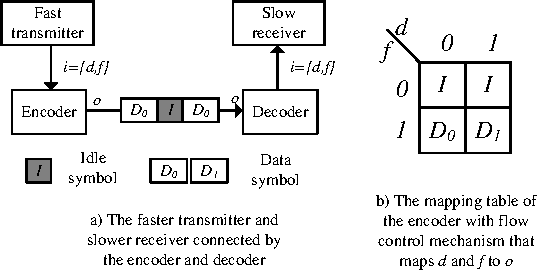
\includegraphics[width=\textwidth]{nonuniq}
\caption{带有流控机制的编码器}
\label{fig_fc}
\end{figure}

\begin{figure}[b]
\centering
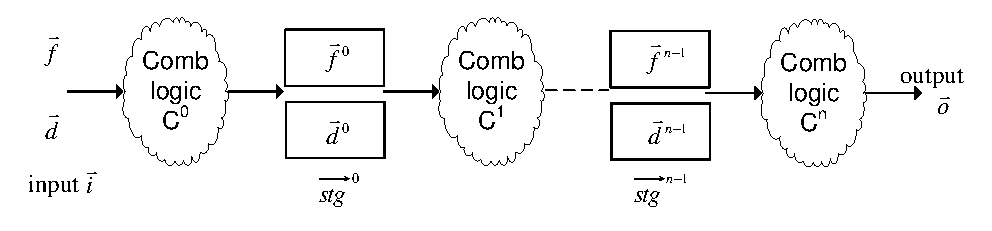
\includegraphics[width=0.9\textwidth]{pipemod1}
\caption{带有流水线和流控机制的编码器}
\label{pipemod}
\end{figure}



同时,
如图\ref{pipemod}所示,
许多编码器
包含流水线级$\vec{stg}^j$ 已将关键的数据路径划分为多个子段$C^j$,
这样有助于提高性能。
类似于$\vec{i}$,
每个流水线级$\vec{stg}^j$ 也可以划分为留空向量$\vec{f}^j$ 和数据向量$\vec{d}^j$。

然而由秦et al. 的算法\cite{QinTODAES15} 产生的解码器并不包含流水线。
这使得其运行速度远低于相应的编码器。
为了解决该问题,
本文提出了一个全新的算法以为此类编码器产生带有流控机制和流水线的解码器。
该算法首先使用秦et al. \cite{QinTODAES15}的算法来寻找$\vec{f}$ 并推导$valid(\vec{f})$。
然后分别通过强制和不强制$valid(\vec{f})$,
已从所有寄存器集合中找到每一个寄存器级$\vec{stg}^j$的$\vec{d}^j$ 和$\vec{f}^j$。
最后通过Jiang et al. \cite{InterpBoolFunction}的算法特征化$\vec{stg}^j$ 和$\vec{i}$的布尔函数。

实验结果表明,
该算法能够为多个工业界的真实编码器正确的产生带有流控和流水线的解码器。

本文剩余部分如下组织。
小节\ref{sec_prem} 介绍相关的背景知识;
小节\ref{sec_framework} 介绍本文算法的整体结构;
小节\ref{sec_pipeinfer} 找到每一个流水线级$\vec{stg}^j$中的$\vec{f}^j$ 和$\vec{d}^j$ 。
小节\ref{sec_char} 为$\vec{stg}^j$ 和$\vec{i}$特征化布尔函数。
小节\ref{sec_exp} 和\ref{sec_relwork} 分别给出实验结果和相关工作。
最后小节\ref{sec_conclude} 给出结论。


\section{背景知识}\label{sec_prem}

% \subsection{Flow control mechanism}\label{subsec_fc}



\subsection{命题逻辑可满足}\label{subsec_SAT}
布尔集合记为$\mathbb{B}=\{0,1\}$。
多个变量组成的向量记为$\vec{v}=(v,\dots)$。
$\vec{v}$ 中的变量个数记为$|\vec{v}|$。
若一个变量$v$ 是$\vec{v}$的成员,
则记为$v\in\vec{v}$;
否则记为$v\notin\vec{v}$。
对于一个变量$v$ 和一个向量$\vec{v}$,
若$v\notin\vec{v}$,
则一个同时包含$v$ 和所有$\vec{v}$ 的成员的新变量记为$v\cup\vec{v}$。
若$v\in \vec{v}$,
则一个包含$\vec{v}$ 的所有成员,但是不包含$v$的
新变量记为$\vec{v}-v$。
对于两个向量$\vec{a}$ 和$\vec{b}$,
则同时包含$\vec{a}$ 和$\vec{b}$ 的所有成员的新向量记为$\vec{a}\cup\vec{b}$。

对于变量集合$V$上的公式$F$,
其命题逻辑可满足问题(SAT)
的目的在于巡展赋值函数$A:V\to \mathbb{B}$,
使得$F$ 能够取值为$1$。
若$A$ 存在则$F$ 是可满足的;
否则是不可满足的。

对于两个布尔命题逻辑公式$\phi_A$ 和$\phi_B$,
若$\phi_A\wedge \phi_B$ 不可满足,
则存在仅引用$\phi_A$ 和$\phi_B$共同变量的公式$\phi_I$ ,
使得$\phi_A\Rightarrow \phi_I$
且$\phi_I\wedge \phi_B$ 不可满足。
$\phi_I$ 称为$\phi_A$ 相对于$\phi_B$的Craig 插值\cite{Craig} 。
可以使用McMillan算法\cite{interp_McMillan} 产生该插值。




\subsection{有限状态机}\label{subsec_fsm}



编码器使用有限状态机$M=(\vec{s},\vec{i},\vec{o},T)$作为模型,
其中包含状态向量$\vec{s}$。
输入向量$\vec{i}$,
输出向量$\vec{o}$,
状态迁移函数$T: \vec{s}\times \vec{i}\to \vec{s}\times \vec{o}$
从当前状态向量和输入向量计算出下一状态向量和输出向量。

$M$ 的行为可以通过展开状态迁移函数进行推导。
状态变量$s\in\vec{s}$, 输入变量$i\in\vec{i}$ 和输出变量$o\in\vec{o}$ 在上述展开序列的第$n$步中
分别记为$s_n$, $i_n$ 和$o_n$。
更进一步的,
在第$n$步中的状态向量,输入向量和输出向量分别记为$\vec{s}_n$, $\vec{i}_n$ 和$\vec{o}_n$。
一个路径是一个序列$<\vec{s}_n,\dots,\vec{s}_m>$ 使得对于所有$n\le j< m$,
有$\exists \vec{i}_j\vec{o}_j (\vec{s}_{j+1},\vec{o}_j)\equiv T(\vec{s}_j,\vec{i}_j)$ 。
而一个环是一个路径$<\vec{s}_n,\dots,\vec{s}_m>$ 使得$\vec{s}_n\equiv \vec{s}_m$。



\subsection{寻找$\vec{f}$的停机算法}\label{subsec_chkextdec}


秦et al. \cite{QinTODAES15} 提出了一个寻找$\vec{f}$ 的停机算法。
该算法通过迭代的调用一个sound和一个complete的算法以最终得到收敛的答案。.
% The first one is an under-approximative one that presented in \ref{subsub_sound},
% while the second one is an over-approximative one presented in \ref{subsub_complete}.
% We will present these two approaches below and show
% that they will eventually converge.

\subsubsection{sound算法}\label{subsub_sound}
如图\ref{fig_pc}a)所示,
在展开的迁移关系上,
一个输入变量$i\in\vec{i}$ 能够被唯一决定,
是指存在$p$, $l$ 和$r$,
使得对于输出序列$<\vec{o}_p,\dots,\vec{o}_{p+l+r}>$的每一个取值,
$i_{p+l}$ 不能同时为0和1。
折等价于公式(\ref{uniqt1})中的$F_{PC}(p,l,r)$的不可满足性。
行1 对应于图\ref{fig_pc}a)中的路径,
而行2 是其拷贝
行3 强制这两个路径的输出相等。
而行4 强制$i_{p+l}$ 不等。
该算法是sound的因为当(\ref{uniqt1}) 不可满足
$i$ 肯定是$\vec{f}$的成员。

\begin{equation}\label{uniqt1}
% \begin{split}
F_{PC}(p,l,r):=
\left\{
\begin{array}{cc}
&\bigwedge_{m=0}^{p+l+r}
\{
(\vec{s}_{m+1},\vec{o}_m)\equiv T(\vec{s}_m,\vec{i}_m)
\}
\\
\wedge&\bigwedge_{m=0}^{p+l+r}
\{
(\vec{s'}_{m+1},\vec{o'}_m)\equiv T(\vec{s'}_m,\vec{i'}_m)
\}
\\
\wedge&\bigwedge_{m=p}^{p+l+r}\vec{o}_m\equiv \vec{o'}_m \\
\wedge& i_{p+l}\equiv 1 \wedge  i'_{p+l}\equiv 0
% \wedge&\bigwedge_{m=0}^{p+l+r}assertion(\vec{i}_m) \\
% \wedge&\bigwedge_{m=0}^{p+l+r}assertion(\vec{i'}_m)
\end{array}
\right\}
% \end{split}
\end{equation}

\begin{figure}[t]
\begin{center}
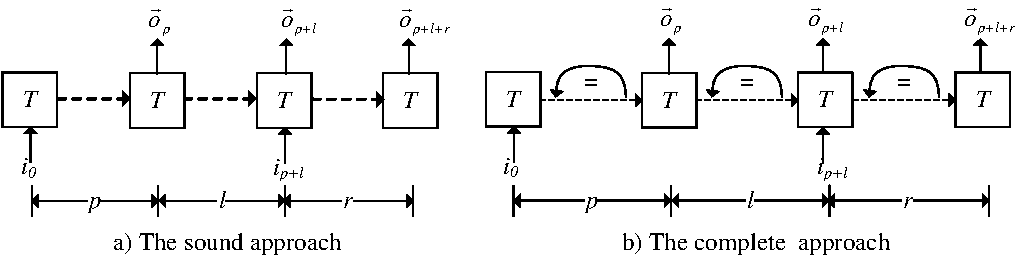
\includegraphics[width=\textwidth]{pc}
\end{center}
\caption{sound和complete方法}
  \label{fig_pc}
\end{figure}


%



\subsubsection{complete算法}\label{subsub_complete}
对于上述的$F_{PC}(p,l,r)$ ,
有两种可能性:
\textbf{(1)}. 存在$p$, $l$ 和$r$,使得$i_{p+l}$ 能够被$<\vec{o}_{p},\dots,\vec{o}_{p+l+r}>$ 唯一决定;
或者\textbf{(2)}. $i_{p+l}$ 对于任意$p$, $l$ 和$r$都不能被唯一决定。


对于第一种情形,
通过迭代的增加$p$, $l$ 和$r$,
$F_{PC}(p,l,r)$ 总能够变成不可满足。
而对于第二种情形,
该算法将永不停机。
因此,
为了得到一个停机算法,
我们需要如图\ref{fig_pc}b) 所示的方法去检查第二种情形。
该方法类似于\ref{fig_pc}a) ,
但是在三个状态序列$<\vec{s}_{0},\dots,\vec{s}_{p}>$, $<\vec{s}_{p+1},\dots,\vec{s}_{p+l}>$ 和
$<\vec{s}_{p+l+1},\dots,\vec{s}_{p+l+r}>$上增加了三个约束用于检测环。
该方法形式化的定义于公式(\ref{uniqln})中。
其中最后三行即为我们新加的三个约束。
该方法是complete,
因为当其是可满足的时候,
我们可以通过展开
这三个环来证明第二种情形并断定 $i\notin \vec{f}$。

\begin{equation}\label{uniqln}
% \begin{split}
F_{LN}(p,l,r):=\\
\left\{
\begin{array}{cc}
&F_{PC}(p,l,r)\\
\wedge&\bigvee_{x=0}^{p-1}\bigvee_{y=x+1}^{p} \{\vec{s}_x\equiv \vec{s}_y\wedge \vec{s'}_x\equiv \vec{s'}_y\} \\
\wedge&\bigvee_{x=p+1}^{p+l-1}\bigvee_{y=x+1}^{p+l} \{\vec{s}_x\equiv \vec{s}_y\wedge \vec{s'}_x\equiv \vec{s'}_y\} \\
\wedge&\bigvee_{x=p+l+1}^{p+l+r-1}\bigvee_{y=x+1}^{p+l+r} \{\vec{s}_x\equiv \vec{s}_y\wedge \vec{s'}_x\equiv \vec{s'}_y\}
\end{array}
\right\}
% \end{split}
\end{equation}


\subsubsection{通过算法\ref{alg_fofc}找到$\vec{f}$ }\label{subsubsec_findfc}

At Line \ref{adduniq},
the input $i$ that can be uniquely determined will be moved to vector $\vec{f}$.
% On the other hand,
If $F_{LN}(p,l,r)$ is satisfiable at Line \ref{nonuniqres},
the input $i$ that can NOT be uniquely determined will be moved to vector $\vec{d}$.
Please refer to \cite{QinTODAES15} for its termination and correctness proof.

\begin{algorithm}[t]
\SetAlgoVlined
\KwIn{The input variable vector $\vec{i}$.}
\KwOut{$\vec{f}\subset \vec{i}$, and the maximal $p$, $l$ and $r$ reached in this searching.}
$\vec{f}: = \{\}$;$\vec{d}:= \{\}$;$p$:= 0 ;~$l$:= 0 ;~$r$:= 0 \;
\ShowLnLabel{while}\While{$\vec{i}\ne \{\}$}{
  assume $i\in\vec{i}$\;
  $p++$; ~ $l++$; ~ $r++$\;
  \uIf {$F_{PC}(p,l,r)$ is unsatisfiable for $i$} {
    \ShowLnLabel{adduniq}
    $\vec{f}:= i\cup\vec{f}$ ; ~
    $\vec{i}:=\vec{i}-i$\;
  }\ShowLnLabel{nonuniqres}
  \ElseIf {$F_{LN}(p,l,r)$ is satisfiable for  $i$}{
    $\vec{d}:=i\cup\vec{d}$ ; ~
    $\vec{i}:=\vec{i}-i$
  }
}
\KwRet ($\vec{f}$, $p$, $l$, $r$)
\caption{Identifying the flow control vector $\vec{f}$}
\label{alg_fofc}
\end{algorithm}


% \section{Inferring the flow control predicate $valid(\vec{f})$}


% Furthermore,
% the validness of $\vec{d}$ is indicated by a predicate $valid(\vec{f})$.
% So for a properly designed encoder,
% $valid(\vec{f})$ should make $\vec{d}$ to be uniquely determined by the encoder's output.

% In Subsection \ref{subsec_craig},
% we propose  an algorithm
% to characterize a Boolean function that makes a Boolean formula satisfiable.
% In Subsection \ref{subsec_infer},
% we apply this algorithm to infer $valid(\vec{f})$,
% % the predicate that enable $\vec{d}$ to be uniquely determined by a bounded sequence of $\vec{o}$.
% the predicate that enables $\vec{d}$ to be uniquely determined.


\subsection{Inferring $valid(\vec{f})$ that enables $\vec{d}$ to be uniquely determined}\label{subsec_infer}
% This subsection introduces the non-trivial details of how to infer the predicate $valid(\vec{f})$.
% So we first present an intuitive and informal introduction in \ref{subsub_intro}.
% And then present its details in \ref{subsub_nonloop}, \ref{subsub_loop} and \ref{subsub_overal}.

% \subsubsection{\textbf{Intuitive introduction}}\label{subsub_intro}.

% In this section,
% we will present how to compute the predicate $valid(\vec{f})$ that enables $\vec{d}$ to be uniquely determined.

This is also proposed by Qin et al. \cite{QinTODAES15}.
It first introduces Algorithm \ref{alg_craigchar} to characterize a function
that makes a Boolean formula satisfiable.
And then as shown in Figure \ref{fig_mono},
Algorithm \ref{alg_craigchar} is used to characterize $\neg FSAT_{PC}(p,l,r)$,
a monotonically growing under-approximation of $valid(\vec{f})$,
and $\neg FSAT_{LN}(p,l,r)$,
a monotonically shrinking over-approximation of $valid(\vec{f})$.
And finally we show that these two approximations will eventually converge to $valid(\vec{f})$.
% Please refer to \cite{QinTODAES15} for the proof of its correctness and termination.



\subsubsection{Characterizing a function that makes a Boolean formula satisfiable}\label{subsubsec_craig}

For a particular Boolean relation $R(\vec{a},\vec{b},t)$,
with $R(\vec{a},\vec{b},0)\wedge R(\vec{a},\vec{b},1)$ unsatisfiable.
Algorithm \ref{alg_craigchar} characterize a Boolean function $FSAT_R(\vec{a})$
that covers and only covers all the valuations of $\vec{a}$
that can make $R(\vec{a},\vec{b},1)$ satisfiable.
Line \ref{testsat} finds out new valuation of $\vec{a}$ that can make $R(\vec{a},\vec{b},1)$ satisfiable,
but hasn't been covered by $FSAT_R(\vec{a})$.
Lines \ref{cofact1}, \ref{cofact2} and \ref{ab} enlarge this valuation
to an interpolant $ITP(\vec{a})$ with McMillan's algorithm \cite{interp_McMillan}.
Line \ref{add} adds $ITP(\vec{a})$ to $FSAT_R(\vec{a})$.
% It is formally defined below:

% we have the following two assumptions:
% \begin{enumerate}
% \item \textbf{Assumption 1} :
% $R(\vec{a},\vec{b},0)\wedge R(\vec{a},\vec{b},1)$ is unsatisfiable.
% % That is,
% % $\vec{a}$ and $\vec{b}$ uniquely determine $t$.
% $\vec{a}$ and $\vec{b}$ are respectively called the important and the non-important variable vectors,
% $t$ is the target variable.
% \item \textbf{Assumption 2} :
% $R(\vec{a},\vec{b},t)$ is satisfiable for all valuations of $\vec{a}$.
% \end{enumerate}
%
% In the remainder of this paper,
% when we use the algorithm introduced in this subsection,
% we will show that these two assumptions are fulfilled.


% \begin{equation}\label{fchar}
% % \begin{split}
% FSAT_R(\vec{a}):=
% \left\{
% \begin{array}{rcl}
% 1 & & \exists\vec{b}.R(\vec{a},\vec{b},1) \\
% 0 & & otherwise
% \end{array}
% \right.
% % \end{split}
% \end{equation}
%% HAHA come to here

% Thus,
% a naive algorithm of computing $FSAT_R(\vec{a})$ is to enumerate all valuations of $\vec{a}$,
% and collect all those valuations that make $R(\vec{a},\vec{b},1)$ satisfiable.
% But the number of valuations to be enumerated is $2^{|\vec{a}|}$,
% which will prevent this algorithm from terminating within reasonable time for a large $\vec{a}$.

% We can speed up this naive algorithm by expanding each valuation of $\vec{a}$
% to a larger set with cofactoring \cite{EFFSATUSMCCO} and Craig interpolant \cite{interp_McMillan}.
% Intuitively,
% assume that $R(\vec{a},\vec{b},1)$ is satisfiable with a satisfying assignment $A:\vec{a}\cup\vec{b}\cup\{t\}\to\{0,1\}$,
% the following new formula can be constructed by cofactoring \cite{EFFSATUSMCCO}:



% \begin{equation}
% % \begin{split}
% R(\vec{a},A(\vec{b}),1):=R(\vec{a},\vec{b},1)_{b\equiv A(b)}
% % \end{split}
% \end{equation}

% Assume $A:\vec{a}\cup\vec{b}\cup\{t\}\to \mathbb{B}$ is a satisfying assignment of $R(\vec{a},\vec{b},1)$.
% % Because $R(\vec{a},A(\vec{b}),0)\wedge R(\vec{a},A(\vec{b}),1)$ is unsatisfiable,
% According to Subsection \ref{subsec_SAT},
% the interpolant $ITP(\vec{a})$ of $R(\vec{a},A(\vec{b}),1)$ with respect to $R(\vec{a},A(\vec{b}),0)$
% % used as an over-approximation of the set of $\vec{a}$ that makes $R(\vec{a},A(\vec{b}),1)$ satisfiable.
% % At the same time,
% % $ITP(\vec{a})\wedge R(\vec{a},A(\vec{b}),0)$ is unsatisfiable,
% % so $ITP(\vec{a})$ covers nothing that can make $R(\vec{a},A(\vec{b}),0)$ satisfiable.
% % Thus,
% covers all $\vec{a}$ that can make $R(\vec{a},A(\vec{b}),1)$ satisfiable.


% Based on the foregoing discussion,

%
% Each iteration of the while loop in Algorithm \ref{alg_craigchar} adds at least a valuation of $\vec{a}$ to $FSAT_R(\vec{a})$,
% which means that $FSAT_R(\vec{a})$ is a Boolean function that covers a bounded and strictly increasing set of valuations of $\vec{a}$.
% So Algorithm \ref{alg_craigchar} is a halting one.


%
% With Algorithm \ref{alg_craigchar} we can find out $FSAT_{F_{PC}}(\vec{f}_{p+l})$,
% the set of
% valuation of $\vec{f}_{p+l}$ that can make $F_{PC}(p,l,r)$ satisfiable for a particular $p$, $l$ and $r$.
% So its negation $\neg FSAT_{F_{PC}}(\vec{f}_{p+l})$ seems to be what we want.
%
% As shown intuitively in Figure \ref{fig_mono},
% $\neg FSAT_{F_{PC}}(\vec{f}_{p+l})$ is an under-approximation of $valid(\vec{f})$
% that grow monotonically with respect to $p$, $l$ and $r$.
% We will prove this in \ref{subsub_nonloop}.
% So we still need an over-approximation of $valid(\vec{f})$
% that shrinks monotonically with respect to $p$, $l$ and $r$ to construct a halting algorithm,
% which will be presented in \ref{subsub_loop}.



% % We call the predicate that cover and only cover this set $FSAT_{PC}(p,l,r)$.
% % And we will present how to infer it in \ref{subsub_nonloop}.
%
% % But as shown in Subsection \ref{subsec_chkextdec},
% % from the fact that $\vec{d}$ is uniquely determined for some particular $p$, $l$ and $r$,
% % we can only know that it is also uniquely determined for all larger $p'$,$l'$ and $r'$.
% % On the other hand,
% But according to Figure \ref{fig_pc} and Proposition \ref{prop_pc1},
% only the unsatisfiability of $F_{PC}(p,l,r)$ can be generalized to larger $p$, $l$ and $r$,
% while its satisfiability can't.
% % $\vec{d}_{p+l}$ not uniquely determined for some particular $p$, $l$ and $r$,
% % may become uniquely determined for larger $p$, $l$ and $r$.
% % For example,
% % an encoder with 3 step latency can't uniquely determine its input $\vec{i}$ with $p$, $l$ and $r$ smaller than 3.
% % But it can with $p$, $l$ and $r$ larger than 3.
% % That means,
% This means,
% a particular valuation of $\vec{f}_{p+l}$ that
% makes $F_{PC}(p,l,r)$ satisfiable for some $p$, $l$ and $r$,
% may make it unsatisfiable for some larger $p$, $l$ and $r$.
%
% So as shown in Figure \ref{fig_mono},
% $FSAT_{F_{PC}}(\vec{f}_{p+l})$ is a set monotonically shrinking with respect to $p$, $l$ and $r$,
% which make its negation $\neg FSAT_{PC}(p,l,r)$ an under-approximation of $valid(\vec{f})$
% that grow monotonically with respect to $p$, $l$ and $r$.
% We still need an over-approximation that shrink monotonically to construct a halting algorithm.


% Inspired by the Figure \ref{fig_ln} and $F_{LN}(p,l,r)$,
% we can compute this over-approximation by using Algorithm \ref{alg_craigchar}
% to find out the set of valuation of $\vec{f}_{p+l}$ that can make $F_{LN}(p,l,r)$ satisfiable.
% We call the predicate that covers and only covers this set $FSAT_{LN}(p,l,r)$.
% With a satisfiable $F_{LN}(p,l,r)$,
% by unrolling the three loops in Figure \ref{fig_ln},
% we can prove that $F_{LN}(p,l,r)$ is still satisfiable for larger $p$, $l$ and $r$.
% That means $FSAT_{LN}(p,l,r)$ is a set of valuation of $\vec{f}_{p+l}$ that makes $F_{LN}(p,l,r)$ satisfiable
% and grows monotonically with respect to $p$, $l$ and $r$.
% So as shown in Figure \ref{fig_mono},
% $\neg FSAT_{LN}(p,l,r)$ is an over-approximation of $valid(\vec{f})$ that shrinks monotonically.
% We will present how to infer it in \ref{subsub_loop}.
%
% Together with these two inferred predicates,
% an iterative algorithm is presented in \ref{subsub_overal} to infer $valid(\vec{f})$.

\begin{algorithm}[t]
\SetAlgoVlined
\KwIn{The Boolean formula $R(\vec{a},\vec{b},t)$.
% its important variable vector $\vec{a}$,
% its non-important variable vector $\vec{b}$,
% and its target variable $t$
}
\KwOut{$FSAT_R(\vec{a})$ that makes $R(\vec{a},\vec{b},1)$ satisfiable.}
\ShowLnLabel{initcondition}
$FSAT_R(\vec{a}):= 0$ \;
\ShowLnLabel{testsat}
\While { $R(\vec{a},\vec{b},1)\wedge\neg FSAT_R(\vec{a})$ is satisfiable } {
  assume $A:\vec{a}\cup\vec{b}\cup\{t\}\rightarrow \{0,1\}$ is the satisfying assignment \;
\ShowLnLabel{cofact1}
  $\phi_A(\vec{a}):= R(\vec{a},A(\vec{b}),1)$ \;
\ShowLnLabel{cofact2}
  $\phi_B(\vec{a}):= R(\vec{a},A(\vec{b}),0)$ \;
\ShowLnLabel{ab}
  assume $ITP(\vec{a})$ is the Craig interpolant of $\phi_A$ with respect to $\phi_B$ \;
\ShowLnLabel{add}
  $FSAT_R(\vec{a}):= ITP(\vec{a}) \vee FSAT_R(\vec{a})$ \;
}
\KwRet $FSAT_R(\vec{a})$
\caption{$CharacterizingFormulaSAT(R,\vec{a},\vec{b},t)$
% :Characterizing a Boolean function over $\vec{a}$ that can make $R(\vec{a},\vec{b},1)$ satisfiable
}
\label{alg_craigchar}
\end{algorithm}

\subsubsection{Computing monotonically growing under-approximation of $valid(\vec{f})$}\label{subsub_nonloop}
By replacing $i$ in Equation (\ref{uniqt1}) with $\vec{d}$ inferred in Algorithm \ref{alg_fofc},
we have:

\begin{equation}\label{uniqt1d}
% \begin{split}
F^d_{PC}(p,l,r):=
\left\{
\begin{array}{cc}
&\bigwedge_{m=0}^{p+l+r}
\{
(\vec{s}_{m+1},\vec{o}_m)\equiv T(\vec{s}_m,\vec{i}_m)
\}
\\
\wedge&\bigwedge_{m=0}^{p+l+r}
\{
(\vec{s'}_{m+1},\vec{o'}_m)\equiv T(\vec{s'}_m,\vec{i'}_m)
\}
\\
\wedge&\bigwedge_{m=p}^{p+l+r}\vec{o}_m\equiv \vec{o'}_m \\
\wedge& \vec{d}_{p+l}\ne \vec{d}'_{p+l} \\
% \wedge&\bigwedge_{m=0}^{p+l+r}assertion(\vec{i}_m) \\
% \wedge&\bigwedge_{m=0}^{p+l+r}assertion(\vec{i'}_m)
\end{array}
\right\}
% \end{split}
\end{equation}

% Here,
% $\vec{d}_{p+l}\ne \vec{d}'_{p+l}$ means some bit in $\vec{d}_{p+l}$
% isn't equal to the corresponding bit in $\vec{d}'_{p+l}$.
If $F^d_{PC}(p,l,r)$ is satisfiable,
then $\vec{d}_{p+l}$ can't be uniquely determined by $<\vec{o}_p,\dots,\vec{o}_{p+l+r}>$.
We define $T_{PC}(p,l,r)$ by collecting the 3rd line of (\ref{uniqt1d}):

\begin{equation}\label{tpc}
% \begin{split}
T_{PC}(p,l,r):=\\
\left\{
\begin{array}{cc}
      &\bigwedge_{m=p}^{p+l+r}\vec{o}_m\equiv \vec{o'}_m \\
\end{array}
\right\}
% \end{split}
\end{equation}

\begin{figure}[b]
\begin{center}
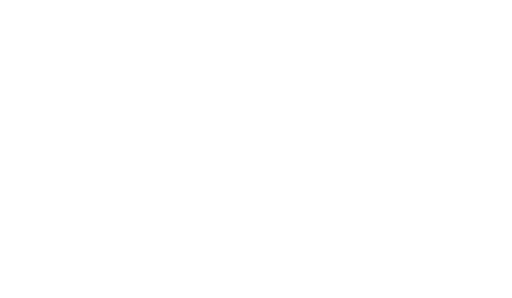
\includegraphics[width=0.5\textwidth]{mono}
\end{center}
\caption{The monotonicity of $FSAT_{PC}(p,l,r)$ and $FSAT_{LN}(p,l,r)$}
  \label{fig_mono}
\end{figure}

By substituting $T_{PC}(p,l,r)$ back into $F^d_{PC}(p,l,r)$,
we have a new formula:
\begin{equation}\label{fpcq}
% \begin{split}
F'^d_{PC}(p,l,r,t):=
\left\{
\begin{array}{cc}
&\bigwedge_{m=0}^{p+l+r}
\{
(\vec{s}_{m+1},\vec{o}_m)\equiv T(\vec{s}_m,\vec{i}_m)
\}
\\
\wedge&\bigwedge_{m=0}^{p+l+r}
\{
(\vec{s'}_{m+1},\vec{o'}_m)\equiv T(\vec{s'}_m,\vec{i'}_m)
\}
\\
\wedge& t\equiv T_{PC}(p,l,r)\\
\wedge& \vec{d}_{p+l}\ne \vec{d'}_{p+l} \\
% \wedge&\bigwedge_{m=0}^{p+l+r}assertion(\vec{i}_m) \\
% \wedge&\bigwedge_{m=0}^{p+l+r}assertion(\vec{i'}_m)
\end{array}
\right\}
% \end{split}
\end{equation}


Obviously $F^d_{PC}(p,l,r)$ and $F'^d_{PC}(p,l,r,1)$ are equivalent.
% $\vec{d}$ cannot be uniquely determined for a particular valuation of $p$, $l$ and $r$ if $F'_{PC}(p,l,r,1)$ is satisfiable.
We further define:

% By comparing Equation (\ref{fpcq}),
% it is obvious that $F_{PC}(p,l,r)$ in Equation (\ref{uniqt1}) can be reformulated as:
% \begin{equation}\label{fpcref}
% % \begin{split}
% F_{PC}(p,l,r):=F'_{PC}(p,l,r,t)\wedge (t\equiv 1)
% \end{equation}
%
% $\vec{f}_{p+l}$ can be uniquely determined by $<\vec{o}_p,\dots,\vec{o}_{p+l+r}>$,
% so $\vec{f}_{p+l}\equiv \vec{f'}_{p+l}$ always holds.
% Thus,
% $\vec{i}_{p+l}\ne \vec{i'}_{p+l}$ in Line 3 of Equation (\ref{fpcq}) should be reformulated as $\vec{d}_{p+l}\ne \vec{d'}_{p+l}$.


% Thus,
% to use Algorithm \ref{alg_craigchar} to characterize the formula over $\vec{f}_{p+l}$ that makes $F'_{PC}(p,l,r,1)$ satisfiable,
% we can define the following equation:
\begin{equation}\label{pcdef1}
\vec{a}:=\vec{f}_{p+l}
\end{equation}

\begin{equation}\label{pcdef2}
\vec{b}:=\vec{d}_{p+l}\cup \vec{d'}_{p+l}\cup \vec{s}_0\cup \vec{s'}_0\cup\bigcup_{0\le x\le p+l+r,x\neq (p+l)}(\vec{i}_{x}\cup\vec{i'}_{x})
\end{equation}

% $\vec{f}_{p+l}$ can be uniquely determined,
% so we don't need to consider $\vec{f'}_{p+l}$.
Thus,
$\vec{a}\cup\vec{b}$ is the vector that contains all the input variable vectors $<\vec{i}_0,\dots,\vec{i}_{p+l+r}>$ and $<\vec{i'}_0,\dots,\vec{i'}_{p+l+r}>$
at all steps for the two sequences of unrolled transition function.
It also contains the two initial states $\vec{s}_0$ and $\vec{s'}_0$.
% In addition,
% the transition function $T$ in the first two lines of Equation (\ref{fpcq})
% is a function that computes the next state and the output variable vector from the current state and input variable vector.
So $\vec{a}$ and $\vec{b}$ can uniquely determine the value of $t$ in $F'^d_{PC}(p,l,r,t)$,
% That is,
% With $\vec{a}$ defined in (\ref{pcdef1}),
% $\vec{b}$ defined in (\ref{pcdef2})
% and $F'^d_{PC}(p,l,r,t)$ as $R(\vec{a},\vec{b},t)$,
which means $R(\vec{a},\vec{b},1)\wedge R(\vec{a},\vec{b},0)$ is unsatisfiable.
Thus,
for a particular combination of $p$, $l$ and $r$,
the Boolean function over $\vec{f}_{p+l}$ that makes $F'^d_{PC}(p,l,r,1)$ satisfiable can be computed
by calling Algorithm \ref{alg_craigchar} with $F'^d_{PC}(p,l,r,t)$, $\vec{a}$ and $\vec{b}$ defined above:

\begin{equation}\label{fsat_pc}
FSAT_{PC}(p,l,r):=CharacterizingFormulaSAT(F'^d_{PC}(p,l,r,t),\vec{a},\vec{b},t)
\end{equation}

% So $FSAT_{PC}(p,l,r)$ is the set of $\vec{f}_{p+l}$
% that makes $F^d_{PC}(p,l,r)$ satisfiable.
% Thus,
% its negation $\neg FSAT_{PC}(p,l,r)$ is the set of $\vec{f}_{p+l}$
% that makes $F^d_{PC}(p,l,r)$ unsatisfiable.
%
% Again according to Proposition \ref{prop_pc1},
% the unsatisfiable proof of $F^d_{PC}(p,l,r)$ can be generalized to all larger $p$, $l$ and $r$.
% So every valuation of $\vec{f}$ covered by $\neg FSAT_{PC}(p,l,r)$ can also make $F^d_{PC}(p,l,r)$ unsatisfiable for all larger $p$, $l$ and $r$.
As shown in Figure \ref{fig_mono},
% we have:
% \begin{proposition}\label{prop_pc}
$\neg FSAT_{PC}(p,l,r)$ is an under-approximation of $valid(\vec{f})$ monotonically growing with respect to
$p$, $l$ and $r$.
% \end{proposition}




\subsubsection{Computing monotonically shrinking over-approximation of $valid(\vec{f})$}\label{subsub_loop}
Similarly,
we can define :
% by replacing $i$ in $F_{LN}(p,l,r)$ of Equation (\ref{uniqln}) with $\vec{d}$,
% we have:
%
% \begin{equation}\label{uniqlnd}
% % \begin{split}
% F^d_{LN}(p,l,r):=\\
% \left\{
% \begin{array}{cc}
% &\bigwedge_{m=0}^{p+l+r}
% \{
% (\vec{s}_{m+1},\vec{o}_m)\equiv T(\vec{s}_m,\vec{i}_m)
% \}
% \\
% \wedge&\bigwedge_{m=0}^{p+l+r}
% \{
% (\vec{s'}_{m+1},\vec{o'}_m)\equiv T(\vec{s'}_m,\vec{i'}_m)
% \}
% \\
% \wedge&\bigwedge_{m=p}^{p+l+r}\vec{o}_m\equiv \vec{o'}_m \\
% \wedge& \vec{d}_{p+l}\ne \vec{d}'_{p+l} \\
% % \wedge&\bigwedge_{m=0}^{p+l+r}assertion(\vec{i}_m) \\
% % \wedge&\bigwedge_{m=0}^{p+l+r}assertion(\vec{i'}_m) \\
% \wedge&\bigvee_{x=0}^{p-1}\bigvee_{y=x+1}^{p} \{\vec{s}_x\equiv \vec{s}_y\wedge \vec{s'}_x\equiv \vec{s'}_y\} \\
% \wedge&\bigvee_{x=p+1}^{p+l-1}\bigvee_{y=x+1}^{p+l} \{\vec{s}_x\equiv \vec{s}_y\wedge \vec{s'}_x\equiv \vec{s'}_y\} \\
% \wedge&\bigvee_{x=p+l+1}^{p+l+r-1}\bigvee_{y=x+1}^{p+l+r} \{\vec{s}_x\equiv \vec{s}_y\wedge \vec{s'}_x\equiv \vec{s'}_y\}
% \end{array}
% \right\}
% % \end{split}
% \end{equation}
%
% If $F^d_{LN}(p,l,r)$ is satisfiable,
% then $\vec{d}_{p+l}$ cannot be uniquely determined by $<\vec{o}_p,\dots,\vec{o}_{p+l+r}>$.
% Furthermore,
% % similar to Proposition \ref{prop_ln1},
% by unrolling those three loops in the last three lines of Equation (\ref{uniqlnd}),
% we can prove that $\vec{d}_{p+l}$ cannot be uniquely determined for any larger $p$, $l$ and $r$.
% We further define a new formula $T_{LN}(p,l,r)$ by collecting the 3rd line and the last three lines of Equation (\ref{uniqlnd}):

\begin{equation}\label{tln}
% \begin{split}
T_{LN}(p,l,r):=\\
\left\{
\begin{array}{cc}
      &\bigwedge_{m=p}^{p+l+r}\vec{o}_m\equiv \vec{o'}_m \\
\wedge&\bigvee_{x=0}^{p-1}\bigvee_{y=x+1}^{p} \{\vec{s}_x\equiv \vec{s}_y\wedge \vec{s'}_x\equiv \vec{s'}_y\} \\
\wedge&\bigvee_{x=p+1}^{p+l-1}\bigvee_{y=x+1}^{p+l} \{\vec{s}_x\equiv \vec{s}_y\wedge \vec{s'}_x\equiv \vec{s'}_y\} \\
\wedge&\bigvee_{x=p+l+1}^{p+l+r-1}\bigvee_{y=x+1}^{p+l+r} \{\vec{s}_x\equiv \vec{s}_y\wedge \vec{s'}_x\equiv \vec{s'}_y\}
\end{array}
\right\}
% \end{split}
\end{equation}

% By replacing the 3rd line and the last three lines of Equation (\ref{uniqlnd}) with $T_{LN}(p,l,r)$,
% we got:

\begin{equation}\label{lndef1}
F'^d_{LN}(p,l,r,t):=
\left\{
\begin{array}{cc}
&\bigwedge_{m=0}^{p+l+r}
\{
(\vec{s}_{m+1},\vec{o}_m)\equiv T(\vec{s}_m,\vec{i}_m)
\}
\\
\wedge&\bigwedge_{m=0}^{p+l+r}
\{
(\vec{s'}_{m+1},\vec{o'}_m)\equiv T(\vec{s'}_m,\vec{i'}_m)
\}
\\
% \wedge& \vec{f}_{p+l}\equiv \vec{f'}_{p+l}\\
\wedge& t\equiv T_{LN}(p,l,r)\\
\wedge& \vec{d}_{p+l}\ne \vec{d'}_{p+l} \\
% \wedge&\bigwedge_{m=0}^{p+l+r}assertion(\vec{i}_m) \\
% \wedge&\bigwedge_{m=0}^{p+l+r}assertion(\vec{i'}_m)
\end{array}
\right\}
\end{equation}

% Obviously $F^d_{LN}(p,l,r)$ and $F'^d_{LN}(p,l,r,1)$ are equivalent.
% Thus,
% with $\vec{a}$ defined in (\ref{pcdef1}),
% $\vec{b}$ defined in (\ref{pcdef2})
% and $F'^d_{LN}(p,l,r,1)$ as $R(\vec{a},\vec{b},t)$,
% we have $R(\vec{a},\vec{b},1)\wedge R(\vec{a},\vec{b},0)$ unsatisfiable.
% Thus,
% for a particular valuation of $p$, $l$ and $r$,
% the function over $\vec{f}_{p+l}$ that makes $F^d_{LN}(p,l,r)$ satisfiable can be
% computed by:

\begin{equation}\label{fsat_ln}
FSAT_{LN}(p,l,r):=CharacterizingFormulaSAT(F'^d_{LN}(p,l,r,t),\vec{a},\vec{b},t)
\end{equation}

% Again according to Proposition \ref{prop_ln1},
% the satisfiable proof of $F^d_{LN}(p,l,r)$ can be generalized to all larger $p$, $l$ and $r$.
% So every valuation of $\vec{f}$ covered by $FSAT_{LN}(p,l,r)$ can also make $F^d_{LN}(p,l,r)$ satisfiable for all larger $p$, $l$ and $r$.
% So $FSAT_{LN}(p,l,r)$ grow monotonically,
% and is a subset of $\neg valid(\vec{f})$.
% Thus we have the following proposition:
As shown in Figure \ref{fig_mono},
% we have:
%
% \begin{proposition}\label{prop_ln}
$\neg FSAT_{LN}(p,l,r)$ is an over-approximation of $valid(\vec{f})$ monotonically shrinking with respect to
$p$, $l$ and $r$.
% \end{proposition}


% It is obvious that $FSAT_{LN}(p,l,r)\to FSAT_{PC}(p,l,r)$.
% Thus,
% for a particular valuation of $p$, $l$ and $r$,
% if $\neg FSAT_{LN}(p,l,r)\wedge FSAT_{PC}(p,l,r)$ is unsatisfiable,
% then $\neg FSAT_{LN}(p,l,r)$ is the formula over $\vec{f}_{p+l}$ that makes $\vec{d}_{p+l}$ to be uniquely determined by the encoder's output sequence.


\subsubsection{Inferring $valid(\vec{f})$ with Algorithm \ref{algo_infer}}\label{subsub_overal}
\begin{algorithm}[t]
\SetAlgoVlined
% \KwIn{The Boolean formula $R(\vec{a},\vec{b},t)$,
% its important variable vector $\vec{a}$,
% its non-important variable vector $\vec{b}$,
% and its target variable $t$.}
% \KwOut{$F_i(\vec{a})$ that makes $R(\vec{a},\vec{b},1)$ satisfiable.}
$p$:= $0$;~$l$:= $0$;~$r$:= $0$ \;
\While { $\neg FSAT_{LN}(p,l,r)\wedge FSAT_{PC}(p,l,r)$ is satisfiable } {
  $p$ ++ ;~$l$ ++ ;~$r$ ++ \;
}
\KwRet {$\neg FSAT_{LN}(p,l,r)$}
\caption{Inferring $valid(\vec{f}_{p+l})$}
\label{algo_infer}
\end{algorithm}

% With these discussion,
% Algorithm \ref{algo_infer} is proposed to infer the predicate $valid(\vec{f}_{p+l})$.
It just iteratively increases the value of $p$, $l$ and $r$,
% until $\neg FSAT_{LN}(p,l,r)\wedge FSAT_{PC}(p,l,r)$ is unsatisfiable,
until $FSAT_{PC}(p,l,r)$ and $FSAT_{LN}(p,l,r)$ converge.
% In this case,
% $\neg FSAT_{PC}(p,l,r)$ is return as $valid(\vec{f})$.
Please refer to \cite{QinTODAES15} for the proofs of its termination and correctness.







第三章研究了拓扑骨干这一低维拓扑特征,本章进一步研究网络受到虫洞攻击引起的异常的高维拓扑特征。虫洞攻击是无线自组织与传感器网络中一种危害严重的攻击。目前已有的大部分虫洞检测机制往往依赖于特殊的硬件设备或较强的网络假设,从而限制了方法的可用性。基于网络拓扑信息的检测方法仅需要利用网络连通性信息,因此具有更好的可用性。现有的基于拓扑信息的方法大致分为两种:基于离散域的局部症状的直接方法,以及基于连续域的全局症状的间接方法。本章深入分析和挖掘虫洞攻击对网络全局拓扑造成的根本影响,结合以上两种基于连通性信息的方法各自的优势,首次提出了一种能够直接在离散域捕获全局的虫洞拓扑症状的检测方法,命名为WormPlanar。WormPlanar的基本思想是基于虫洞攻击对网络的平面化特征造成的根本影响,巧妙地将平面化技术应用于虫洞攻击的检测。本章从理论上证明了方法的正确性,被通过大量的仿真实验验证了方法的性能。
\section{引言}
虫洞攻击是无线自组织与传感器网络中一种危害严重的攻击\upcite{wormhole_cnds05,wormhole_icnp02}。在虫洞攻击中,攻击者在网络中距离较远的两点之间建立优质高速的虫洞链路,使得虫洞两端的节点错误地认为彼此距离很近并通过虫洞链路传输数据包。图\ref{fig:401a}给出了虫洞攻击的示意图,其中$A$和$B$ 表示攻击者部署的两个虫洞收发器,灰色区域表示虫洞天线的影响范围。攻击者利用虫洞天线捕获物理层的无线信号,通过虫洞链路发送到另一端,并在另一端进行广播。虫洞两端的节点将错误地认为彼此是距离很近的直接邻居。本章中统一地将虫洞天线影响范围内的节点称为虫洞节点,如图\ref{fig:401a}中的\{3,4,5,6,7\} 和\{13,14,15,16\}分别是两端的虫洞节点,将虫洞节点之间的虚拟的通讯链路称为虫洞链路。节点在进行路由决策时,将优先地选择这些虫洞链路。借此,攻击者就能够捕获大量的网络数据包,并发动多种攻击,如选择性地丢包、篡改包、乱序发送等。通过收集并分析大量的数据包,攻击者还可以进一步发动更严重的攻击,如协议分析、密码破解、中间人攻击等。虫洞攻击从根本上改变了网络的拓扑结构,从而极大地危害网络中的各种协议和功能,包括路由、定位、拓扑控制等。另外,攻击者能够在不破坏任何合法节点或密码机制的情况下发动虫洞攻击,使得传统的基于密码学的安全机制无法解决虫洞攻击\upcite{wormhole_infocom03}。
\begin{figure}[t]
  \centering
  \subfloat[虫洞攻击的示例]{
    \label{fig:401a}
    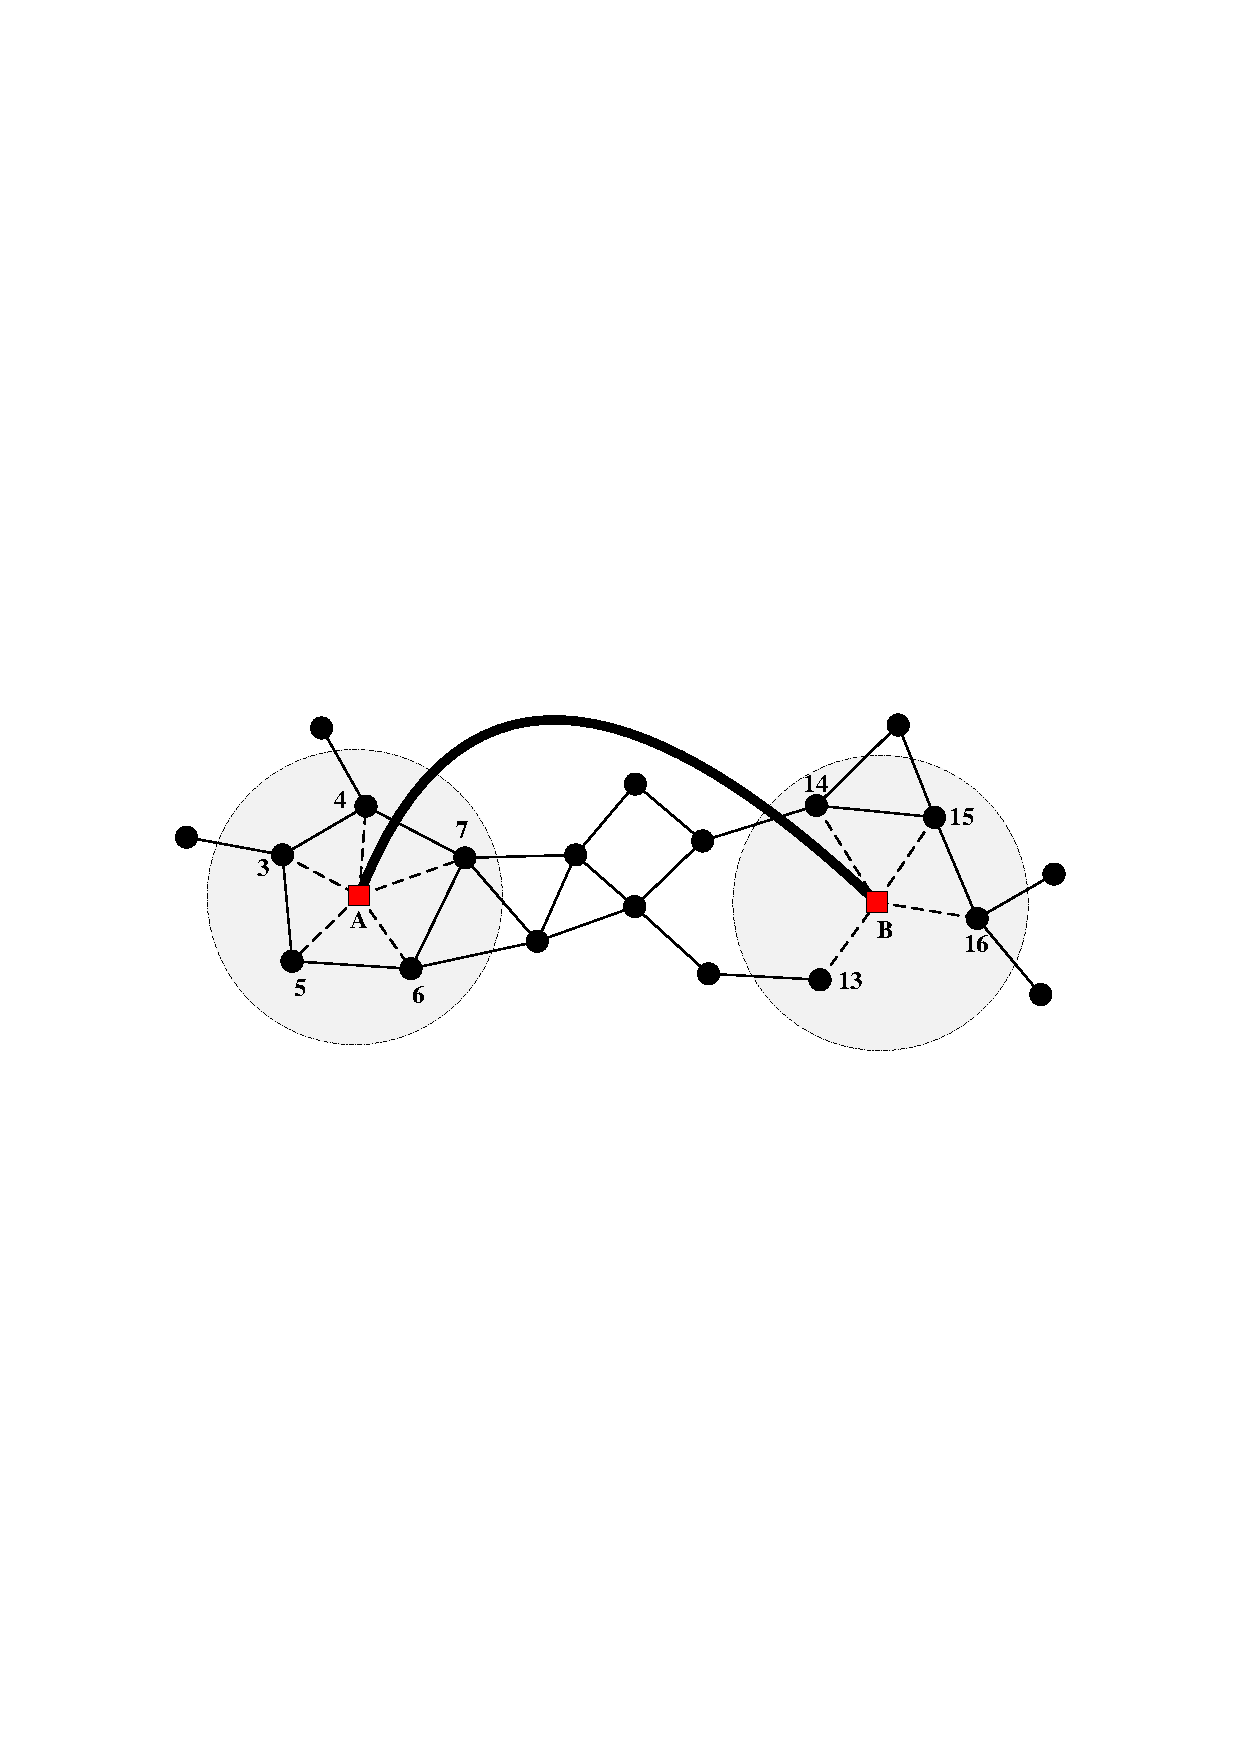
\includegraphics[width=.55\textwidth]{fig401-a}}\hspace{1em}
  \subfloat[虫洞的局部拓扑结构]{
    \label{fig:401b}
    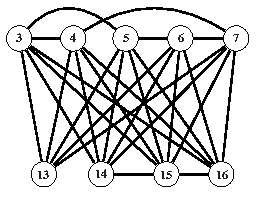
\includegraphics[width=.3\textwidth]{fig401-b}}
  \caption{虫洞攻击的示例及其局部拓扑结构}
  \label{fig:401}
\end{figure}

虫洞攻击近年来成为无线自组织和传感器网络中的研究热点,研究者提出了大量不同类型的虫洞检测机制\upcite{wormhole_cnds05,wormhole_icnp02,wormhole_infocom03,wormhole_wwcmc,wormhole_sasn03,wormhole_icnp06,wormhole_ndss04,wormhole_wise04,wormhole_infocom07,wormhole_mobihoc11,wormhole_ton,wormhole_icnp09,wormhole_icpads09}。
目前已有的虫洞检测方法大部分依赖于专门的硬件设备或较强的网络假设。例如,有些方法需要使用特殊的硬件设备,如GPS\upcite{wormhole_infocom03,wormhole_wwcmc}、 定向天线\upcite{wormhole_ndss04}、 特殊的无线收发模块\upcite{wormhole_sasn03}等,但额外的硬件将增加系统的成本和能量开销;有些方法依赖于理想的网络假设,如全网的精确时钟同步\upcite{wormhole_infocom03}、专门的警卫节点\upcite{wormhole_poovendran}、 安全的初始环境\upcite{wormhole_ipdps05,wormhole_ESAS,wormhole_liteworp,wormhole_mobiworp} 等。对专门的硬件设备和较强的网络假设的依赖限制了这些方法的可用性。为了改善方法的可用性,研究者提出了基于网络拓扑的虫洞检测方法,仅利用连通性信息来检测虫洞攻击。这些方法主要分为两类,分别是基于离散域的局部洞症状的直接方法\upcite{wormhole_wise04,wormhole_infocom07,wormhole_mobihoc11} 和基于连续域的全局症状的间接方法\upcite{wormhole_icpads09,wormhole_ton,wormhole_icnp09}。 直接的方法比较简单,但往往是基于局部拓扑特征的启发式方法,因此检测的准确性缺乏理论上的证明。间接的方法在连续域分析虫洞的全局的本质特征,其正确性在理论上可证明,但检测性能受限于将连续域观察结果扩展至离散网络中检测算法时可能产生的失真。目前还没有一种有效的基于连通性信息的检测方法,能够直接在离散网络中捕获虫洞的全局拓扑症状。综上所述,虫洞检测问题虽然已经得到了长时间的研究,也产生了大量的研究成果,但是依然没有得到充分的解决。

\begin{figure}[t]
  \centering
  \subfloat[正常的网络连通图]{
    \label{fig:402a}
    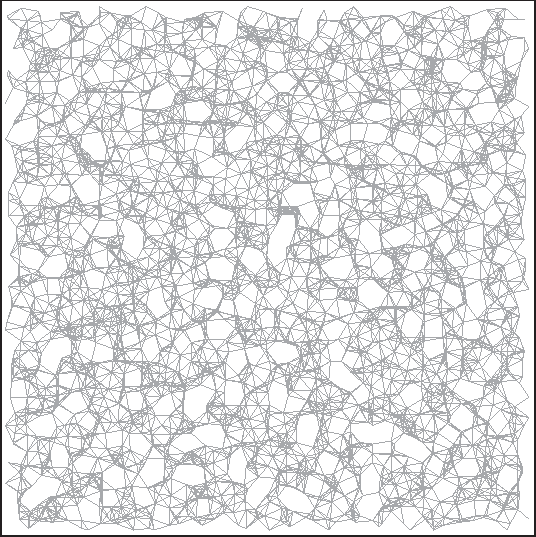
\includegraphics[width=.45\textwidth]{fig402-a}}\hspace{0.5em}%
  \subfloat[平面化子图]{
    \label{fig:402b}
    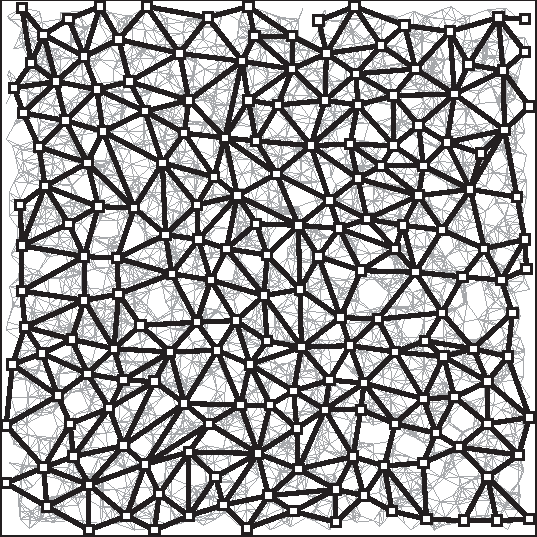
\includegraphics[width=.45\textwidth]{fig402-b}}\hspace{0.5em}%
     \subfloat[包含虫洞的网络连通图]{
    \label{fig:402c}
    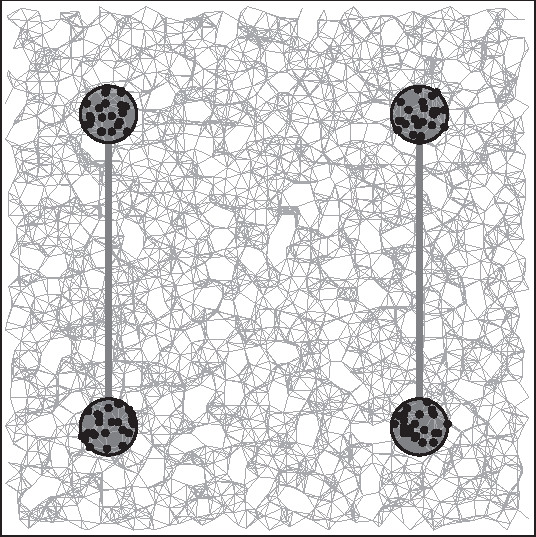
\includegraphics[width=.45\textwidth]{fig402-c}}\hspace{0.5em}%
  \subfloat[平面化处理的结果]{
    \label{fig:402d}
    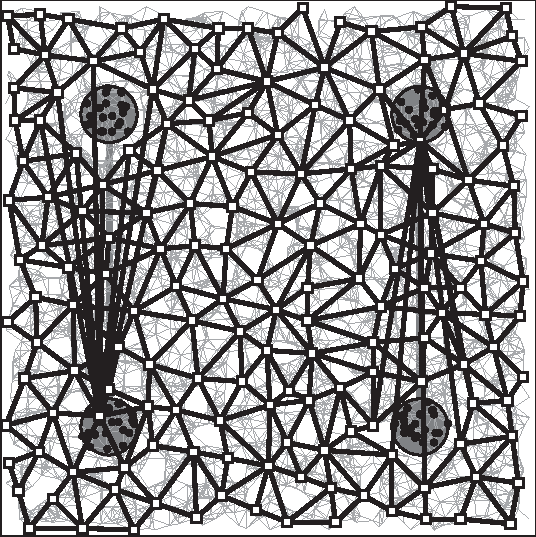
\includegraphics[width=.45\textwidth]{fig402-d}}
  \caption{虫洞攻击对网络平面化技术的影响}
  \label{fig:402}
\end{figure}
本章深入地分析虫洞攻击对网络全局拓扑造成的根本影响,致力于挖掘出一种可以直接用离散域的拓扑信息来描述的全局性的虫洞症状。本章工作的基本思想来自于对网络平面化问题的一个重要观察结果:对于一个正常的网络连通图,利用文献\upcite{planar_tmc}中的平面化算法始终可以提取出一个平面化的子图;而当网络中存在虫洞时,算法无法得到平面化的结果。图\ref{fig:402}中的实例直观地描述了虫洞攻击对网络平面化造成的影响。图\ref{fig:402a}给出了一个正常的网络连通图,其中2500个节点部署在正方形区域内,平均节点度为8.93。图\ref{fig:402b}表示对该网络连通图应用平面化算法得到的结果,其中小正方形和粗线分别表示平面化子图的点和边。图\ref{fig:402c}给出一个包含虫洞的网络连通图,其中灰色圆形区域表示虫洞天线的影响范围,黑色圆点表示虫洞节点,灰色粗线代表虫洞链路(为便于观察没有逐条画出)。图\ref{fig:402d}中粗线表示对包含虫洞的网络连通图执行平面化处理得到的结果,可见结果所示子图是非平面化的。基于以上重要的观察结果,本章提出通过验证网络的可平面性(planarity)来检测潜在的虫洞,并设计了称为WormPlanar的虫洞检测算法。首先,每个节点收集局部的邻居信息,并对局部邻居子图应用优化的平面化算法。若算法能够得到平面化的结果,则该节点为正常节点,否则将该节点标记为疑似虫洞节点。接下来,算法执行修正过程,利用本章提出的判断虫洞链路的两个必要条件,对疑似虫洞节点进行过滤以排除误报的情况。WormPlanar算法仅利用局部连通性信息,巧妙地利用网络平面化技术,首次实现了直接在离散网络中捕获全局的虫洞症状。本章从理论上对算法的正确性进行了严密的证明,并通过大量的仿真实验验证了算法的性能。

本章余下的部分组织如下:4.2节介绍本章采用的网络模型和虫洞攻击模型;4.3节介绍WormPlanar方法的具体设计,并给出必要的理论证明;4.4节通过大量的仿真实验检验方法的有效性和性能;最后4.5节对本章进行总结。
\section{问题描述}
本节阐述基本的网络配置和假设,分别介绍了本章采用的网络模型和假设,以及虫洞攻击模型。
\subsection{网络模型}
本章考虑部署在平面区域上的无线传感器网络,假设网络中每个节点有唯一ID。我们将网络通讯的连通关系图建模为一个简单无向图$G(V,E)$,其中点集$V$表示传感器节点,边集$E$表示节点之间直接的通讯链路。网络中所有的节点不需要装备特殊的硬件设备,也不要求实现全局的严格时钟同步。本章所提出的算法中需要利用已有的网络平面化算法\upcite{planar_tmc},该算法的理论证明是在Q-UDG图模型下完成,且要求参数为$\rho\ge1/\sqrt{2}$,因此本章也采用同样的假设。需要指出的是,本章所提出的算法并不依赖于特定的网络图模型,大量的仿真实验结果也证明了算法在一般的图模型下仍然有效。

另外,本章假设网络中节点能够收集自身的$k$跳邻居信息,获得局部的$k$跳邻居子图。一般情况下,参数$k$ 仅需设置为较小的常数,例如$k$=5就能够满足本章所涉及到绝大部分网络实例的需求。在本章中,$N_G^k(v)$ 表示点$v$的$k$跳以内的邻居集合;$G(X)$表示由点集$X$中所有的点以及它们之间的边构成的子图;点$v$的$k$跳邻居子图就可以表示为$G_k(v)=G(N_G^k(v)\cup{v})$。
\subsection{攻击模型}
本章采用之前研究中广泛采用的基本的虫洞攻击的假设。攻击者只需要获得发动虫洞攻击所需要的最小能力。具体来讲,攻击者不需要攻破任何网络节点或获得网络中相关协议的信息,攻击者部署的虫洞收发设备不需要获得合法的网络ID。虽然虫洞攻击可以从物理层或链路层上改变网络的邻居发现机制,从而显著地改变网络的连通性拓扑,但通过加密网络协议传输的数据本身对于攻击者来说仍然是不可获得的。对于图\ref{fig:401a}中所示虫洞攻击的示例,图\ref{fig:401b}给出了虫洞节点构成的局部拓扑结构。可见,虫洞节点以及虫洞链路实际上构成了一个完全二部图结构,这一特性对于设计虫洞检测算法的设计具有重要的作用,本章后面的部分将进行具体介绍。定义\ref{def:401}\upcite{dong}对一般化的虫洞攻击进行了形式化的描述。
\begin{definition}\label{def:401}
设$G$为网络连通图,$w$为网络中的一种攻击,$G_w$为攻击$w$发生后的网络连通图,$L(u,v)$和$L_w(u,v)$分别表示任意一对顶点$u,v\in{V(G)\cap{V(G_w)}}$在$G$ 和$G_w$中的最短路径。如果$L_w(u,v)<L(u,v)$,则称$G_w$处于虫洞攻击中;设$\lambda_{uv}=L(u,v)-L_w(u,v)$,虫洞攻击$w$的攻击强度定义为$\lambda=max\{\lambda_{uv}|u,v\in{V(G)\cap{V(G_w)}}\}$。
\end{definition}

攻击强度描述了虫洞攻击引起的拓扑变化的程度。本章也将虫洞攻击强度$\lambda$称为虫洞的长度,并假设仅需要检测长度大于一定门限值$\delta$的虫洞,即$\lambda\ge\delta$。一般情况下,虫洞越长所造成的影响范围越大,危害也越严重,较短的虫洞由于影响范围有限,危害也较轻。具体来讲,本章假设所要求检测的虫洞长度的门限值为$\delta=8$,因为这一设置比较适用于当前的无线自组织和传感器网络的规模。除此之外,本章对虫洞攻击模型不再做任何额外的假设和限制。
\section{WormPlanar虫洞拓扑识别方法设计}
本节介绍不依赖位置信息的虫洞拓扑识别方法WormPlanar的具体设计,并从理论上证明方法的正确性。首先概述方法的基本思想和主要过程,然后分别对方法中重要的步骤进行详细的介绍,最后给出具体的算法,并对算法中一些关键的参数及其对算法性能的影响进行讨论。
\subsection{方法概述}
在仅给定连通性信息而不对网络连通图做任何额外限制的情况下,仅从图论的角度无法将虫洞链路和一般的链路区别开。但实际上一个正常的无线传感器网络的连通图并不是一个任意的图,而是具有某种固有的几何结构,这种几何结构来自于网络底层的低维部署区域。网络内在的几何属性被广泛地应用于无线传感器网络中各种高效协议的设计,包括地理路由、拓扑发现、虫洞检测等。例如,文献\upcite{wormhole_ton}提出将网络连通图建模成连续的流形曲面,在连续域中对虫洞造成的影响进行分析。该方法的主要思想是将高维的网络连通图转化至更容易分析的低维空间,同时保留虫洞造成的异常特征。但是该方法的主要局限性在于需要将连续域的分析结果扩展至离散网络中具体的协议,而在此过程中可能引入一定的失真和网络开销。在本章的工作中,我们致力于避免在连续域和离散域之间进行切换,而直接在离散域将网络连通图和网络的几何属性相结合。本章提出的WormPlanar方法在仅利用局部连通性信息的情况下,直接在离散域捕获全局的虫洞症状。WormPlanar 方法的基本思想是利用虫洞链路对网络全局拓扑的可平面性造成的影响,利用已有的基于连通性信息的平面化技术来检测潜在的虫洞。
\begin{figure}[t]
  \centering
  \subfloat[包含虫洞链路的网络连通图]{
    \label{fig:403a}
    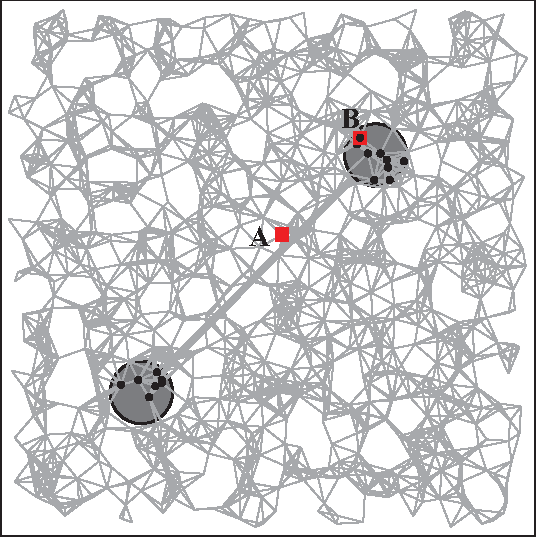
\includegraphics[width=.45\textwidth]{fig403-a}}\hspace{0.5em}%
  \subfloat[WormPlanar检测结果]{
    \label{fig:403b}
    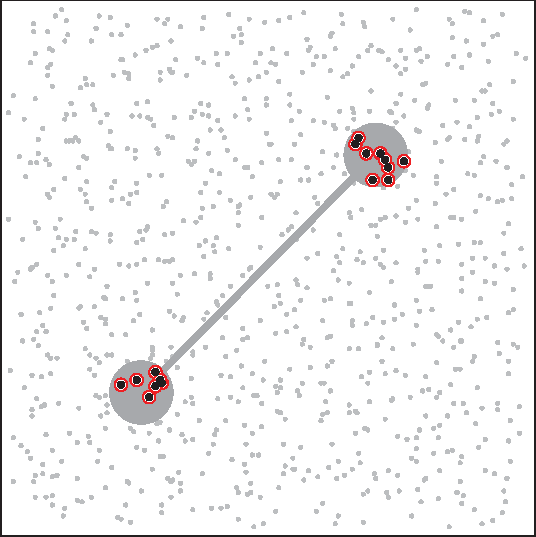
\includegraphics[width=.45\textwidth]{fig403-b}}\hspace{0.5em}%
  \subfloat[MDS-VOW检测结果]{
    \label{fig:403c}
    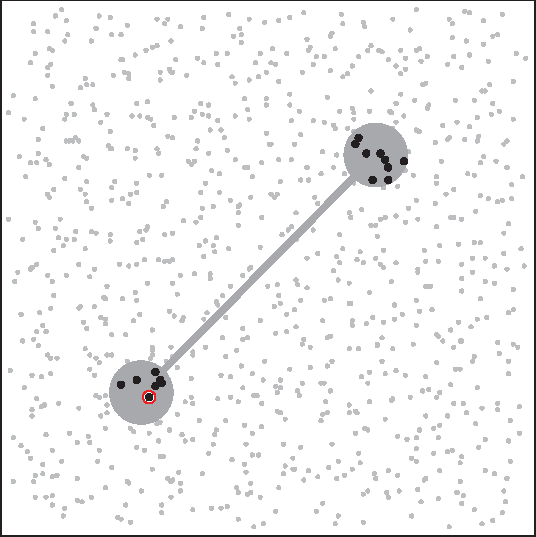
\includegraphics[width=.45\textwidth]{fig403-c}}\hspace{0.5em}%
  \subfloat[LCT检测结果]{
    \label{fig:403d}
    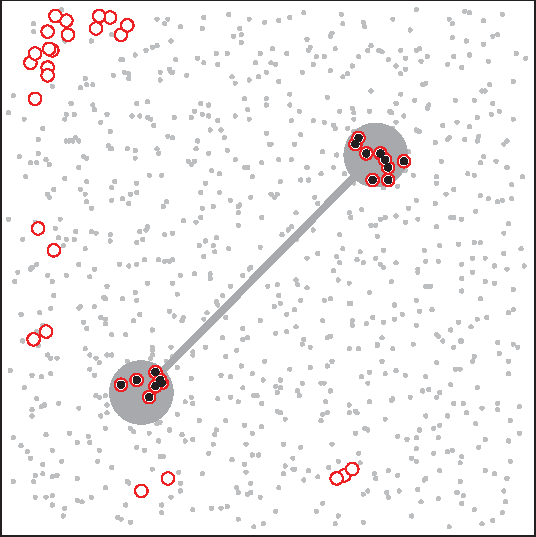
\includegraphics[width=.45\textwidth]{fig403-d}}\hspace{0.5em}%
  \caption{WormPlanar方法与其它方法检测结果的比较}
  \label{fig:403}
\end{figure}

\begin{figure}[t]
  \centering
  \subfloat[$A$点的邻居子图]{
    \label{fig:404a}
    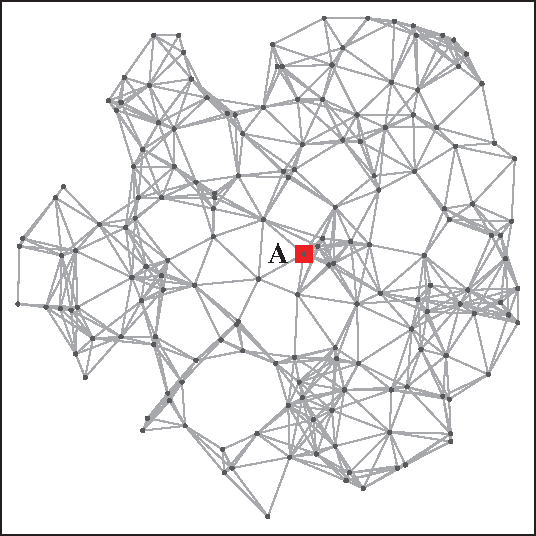
\includegraphics[width=.45\textwidth]{fig404-a}}\hspace{0.5em}%
  \subfloat[$B$点的邻居子图]{
    \label{fig:404b}
    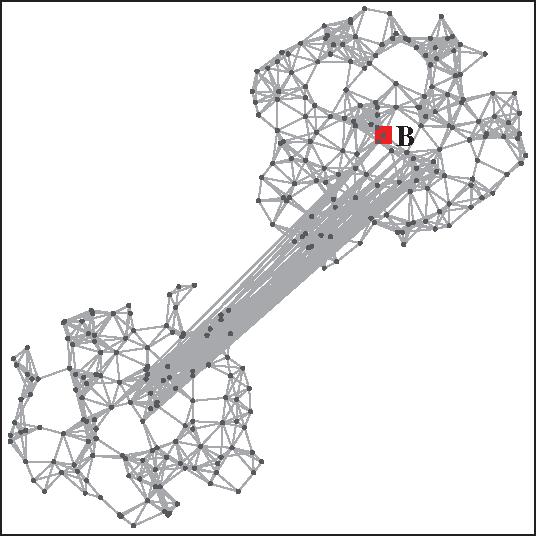
\includegraphics[width=.45\textwidth]{fig404-b}}\hspace{0.5em}%
  \subfloat[$A$点的平面化结果]{
    \label{fig:404c}
    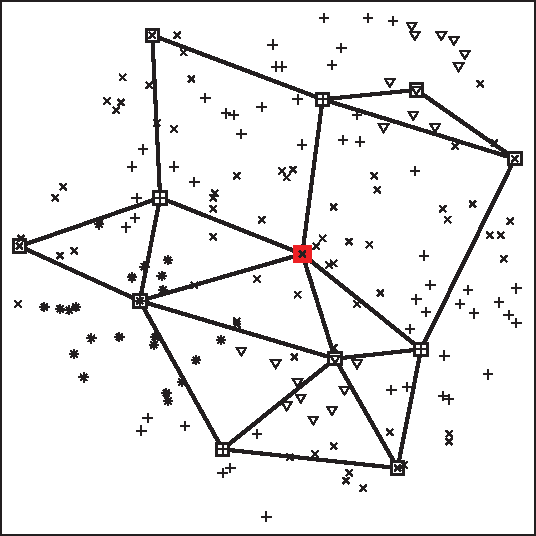
\includegraphics[width=.45\textwidth]{fig404-c}}\hspace{0.5em}%
  \subfloat[$B$点的平面化结果]{
    \label{fig:404d}
    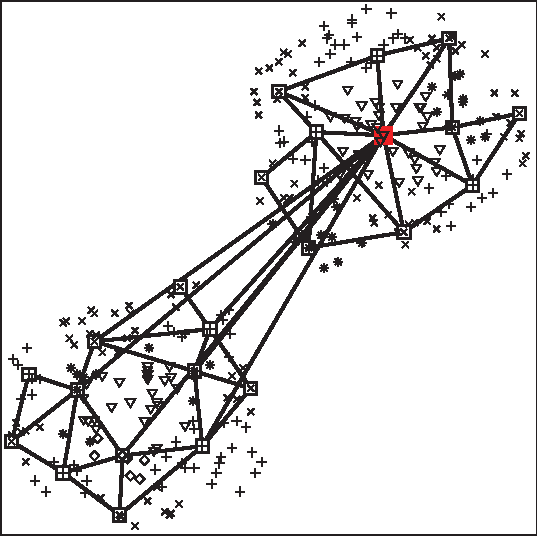
\includegraphics[width=.45\textwidth]{fig404-d}}
  \caption{WormPlanar方法的执行实例}
  \label{fig:404}
\end{figure}
网络拓扑的可平面性是一种全局的属性,并且通过离散的连通性信息来描述。现有的网络平面化算法有很多,但是往往无法有效地捕获虫洞对网络的可平面性造成的本质影响。具体来讲,由于无法将虫洞链路和一般的链路区分开,平面化算法很可能在执行过程中将虫洞链路删除,从而导致虫洞症状的消失,也就无法实现虫洞的检测。然而,文献\upcite{planar_tmc}中提出的TPS平面化算法具有进行虫洞检测所需要的特性。对于任意给定的网络连通图,TPS算法按照一定的规则选择性地删除某些局部连通性,同时又能够保留全局的拓扑特征,比如保证了较长的虫洞链路不会被删除。本章提出的WormPlanar方法对TPS算法进行了定制的修改,使得其更适用于虫洞检测应用。然而,如果直接将该算法应用于整个网络的连通图,虽然能够判定网络中是否存在虫洞,却无法准确地定位虫洞节点和虫洞链路。为了解决这一问题,我们提出将TPS算法应用于每个节点的局部邻居子图,通过检验邻居子图的可平面性来判断该节点是否为潜在的虫洞节点。然后,再利用本章所提出的判定虫洞链路的两个必要条件对疑似虫洞节点进行过滤,移除可能存在的误报的情况。至此,WormPlanar实现了准确地检测和定位虫洞节点和虫洞链路,并进一步对其进行隔离以消除虫洞效应。

为了直观地表示WormPlanar相对于之前方法的优势,图\ref{fig:403}给出了一个具体的实例。图\ref{fig:403a}表示一个包含了虫洞链路的网络连通图,其中900个节点部署在一个正方形区域内,平均节点度为8.85。$A$和$B$分别是一个正常的节点和一个虫洞节点。图\ref{fig:403b}给出了WormPlanar方法的检测结果,其中黑点表示实际的虫洞节点,圆圈表示算法检测出的虫洞节点。可见,WormPlanar准确地检测出了所有的虫洞节点,且没有误报的情况。图\ref{fig:403c}表示利用文献\upcite{wormhole_wise04}中的MDS-VOW方法得到的检测结果,大部分的虫洞节点没有被检测出。这是因为MDS-VOW方法仅适用于两端各有一个虫洞节点的特殊情况,而无法处理一般的虫洞模型。图\ref{fig:403d}表示利用文献\upcite{wormhole_mobihoc11}中的LCT方法得到的检测结果。虽然所有的虫洞节点都被检测出,但同时产生了大量误报的情况。这是由于LCT方法仅基于局部的连通性特征来判断虫洞节点,因此检测的准确性受到具体的网络情况的显著影响。

WormPlanar方法主要包括两个组件:(1)局部可平面性检验;(2)修正过程。下面通过图\ref{fig:404}所示的具体实例对方法的主要过程进行概述。在局部可平面性检验中,每个节点通过收集局部邻居信息获得自身的$k$跳邻居子图,并调用平面化算法对局部邻居子图进行处理。然后检验平面化处理结果的平面性,若结果是平面化的则将该节点标记为正常节点,否则标记为疑似虫洞节点。例如,图\ref{fig:404a}-\ref{fig:404b}分别表示图\ref{fig:403a}中所示的正常节点$A$和虫洞节点$B$ 的5 跳邻居子图。对两个邻居子图分别进行平面化处理,得到图\ref{fig:404c}-\ref{fig:404d}所示的结果,其中正方形和粗线分别表示结果中的点和边。显然,节点$A$ 得到的结果是平面的,因此被标记为正常节点;节点$B$得到的结果则是非平面的,因此被标记为疑似虫洞节点。网络中所有的节点以分布式的方式执行局部可平面性检验,从而检测出所有的疑似虫洞节点。在检测出所有的疑似虫洞节点后,WormPlanar进入第二个主要过程,即修正过程。在修正过程中,方法对疑似虫洞节点进行过滤以移除在局部可平面性检验过程中可能产生的误报。例如,某些距离虫洞节点比较近的正常节点,由于它们的局部邻居子图中可能包含虫洞节点和虫洞链路,无法通过局部可平面性检验,因此被错误地标记为疑似虫洞节点。较高的误报率将导致大量的正常节点和链路被隔离,从而显著地影响网络的连通性和能力。误报在之前的研究\upcite{wormhole_mobihoc11}中是一个难以解决的问题,在本章的工作中得到了很好的解决,本章后面的实验部分还将具体介绍。为了解决误报问题,我们深入地研究虫洞攻击对网络连通性造成的根本影响,提出了判定虫洞链路的两个必要条件,并利用这两个条件对疑似虫洞节点进行过滤从而移除误报。

接下来对WormPlanar方法的两个主要组件分别进行详细的介绍,并给出必要的证明过程。
\subsection{局部可平面性检验}
为了叙述的方便,下面将局部可平面性检验组件进一步划分为三个阶段,并分别进行介绍。
\subsubsection{构建邻居子图}
首先,网络中的每个节点收集局部邻居信息,获得自身的$k$跳邻居子图。这一过程可以通过一个简单的局部洪泛消息来实现。每个节点$v$向自己的直接邻居发送一条洪泛消息,消息中包含本节点的直接邻居列表和代表消息经历跳数的计数器。消息每被转发一次,计数器的值增加1,增加至$k$时消息停止转发。洪泛消息完成后,每个节点$v$都可以获得自身$k$跳以内的邻居列表$N_G^k(v)$以及它们的直接邻居信息,从而构建出$k$跳邻居子图$G_k(v)$。
\subsubsection{执行平面化算法}
完成邻居子图的构建后,每个节点调用平面化算法TPS对邻居子图进行处理。下面对平面化算法TPS中的相关定义和大致过程进行介绍。首先,算法从邻居子图中提取出一个RWG(restricted witness graph)图,如定义\ref{def:402}\upcite{planar_infocom11}所述。对于给点的网络连通图$G$,以及顶点集合$X,Y$,$D(G)$表示图$G$的直径,即图中任意两个顶点之间的最短距离的最大值;$d_G(X,Y)$表示点集$X,Y$在图$G$中的距离,即$X$中任意顶点和$Y$中任意顶点之间的最短路径长度的最小值。

\begin{definition}\label{def:402}
给定网络连通图$G(V,E)$,以及两个正整数$\alpha,\beta$,图$G$中的一个$(\alpha,\beta)$-RWG 图表示为$G_{RWG}$,其定义如下:(1)$G_{RWG}$中每个顶点$v_i$对应于顶点集$V(G)$的一个子集$V_i$,且满足$D(G(V_i))\le\alpha, \bigcup_{v_i\in{V(G_{RWG})}}V_i=V(G)$;(2)$G_{RWG}$中存在一条边$(v_i,v_j)$当且仅当$d_G(V_i,V_j)\le\beta$。
\end{definition}

本章所采用的RWG图的构建过程如下所述。首先,从顶点集$V(G)$中选择一个$\tau$跳独立集作为地标节点集,同时作为RWG图中的顶点。$k$跳独立集定义为满足如下两个条件的顶点集合$V$:(1)$\forall{v_i,v_j}\in{V}, d_G(v_i,v_j)>\tau$;(2)向$V$中加入任何新的顶点将不再满足条件(1)。在本章的工作中,$\tau$被设置为固定的常数2。然后,剩余的所有节点将被分配给距离自己最近且ID最小的地标节点。这样,整个网络连通图被划分为一组类Voronoi 分区。接下来构造RWG图中的边。若两个地标节点所在的分区中存在共享同一条边的两个顶点,则在这两个地标节点之间连一条边,并作为RWG图中的边。至此,所有的地标节点以及它们之间的边就构成了一个RWG图,确切地说是$(2\tau,1)$-RWG图。

然后调用平面化算法TPS,按照一定的原则对RWG图中的边进行修剪操作,得到一个子图。文献\upcite{planar_tmc}中证明了对于任意给定的正常的网络连通图,利用TPS 算法提取出的子图一定是连通的平面化图。图\ref{fig:404c}表示利用平面化算法对图\ref{fig:404a}中所示的点$A$的邻居子图进行处理后的结果,其中正方形表示RWG图中的顶点,不同的符号代表位于不同Voronoi分区内的顶点,正方形之间的连线表示平面化处理后的边。显然,该子图是平面的。为了使平面化算法更好地体现虫洞造成的非平面化特征,我们对算法进行了一些改进。在对节点$v$的邻居子图$G_k(v)$ 进行处理时,强制地指定$v$为一个地标节点,并将$v$ 的两跳以内的邻居分配给$v$。利用这一设置,当$v$为一个虫洞节点时,其所在分区就能够包含该虫洞攻击中所有的虫洞节点。这一特性将有利于形成可证明的非平面化结构,后面还将对这一问题进行详细的阐述。图\ref{fig:404b}给出了一个虫洞节点$B$的5跳邻居子图,而图\ref{fig:404d}表示对该图进行平面化处理后得到的结果,显然该结果是非平面化的。但是如何对其非平面性进行验证,这是下一个组件所要完成的工作。
\subsubsection{验证平面性}
执行完平面化算法后,接下来对结果的平面性进行验证,并根据验证结果对疑似虫洞节点进行判定。

首先结合以上观察结果以及文献\upcite{planar_infocom11}中证明过的定理\ref{theorem401},我们可以直接地得到定理\ref{theorem402}。
\begin{theorem}
  \label{theorem401}
利用平面化算法TPS获得的结果一定是平面图。
\end{theorem}

\begin{theorem}
  \label{theorem402}
对于满足$\rho\ge1/\sqrt{2}$的Q-UDG图$G$中的任意顶点$v$,如果TPS算法无法从邻居子图$G_k(v)$中得到平面化子图,则图$G_k(v)$中一定包含虫洞。
\end{theorem}

定理\ref{theorem402}中设置$\rho\ge1/\sqrt{2}$的Q-UDG图的条件是因为文献\upcite{planar_infocom11} 中的证明过程采用了这一假设,而这也是无线自组织和传感器网络研究中常用的假设条件。根据以上观察结果以及定理\ref{theorem401}和定理\ref{theorem402},我们初步地将所有无法获得平面化结果的节点标记为疑似虫洞节点。在此过程中,仍有一个重要的问题需要解决,即如何准确地判定平面化算法的结果是否为平面图。为了解决这一问题,我们提出了平面性判定准则,如定理\ref{theorem403}所述。给定网络连通图$G$,假设$\Gamma(v)$表示对顶点$v$的局部邻居子图执行平面化处理后的结果,$N_{\Gamma}^1(v)$表示$v$ 在$\Gamma(v)$中的直接邻居集合。图$G$中的简单环$C$定义为$G$中一个连通的、每个节点的度均为2的子图。假设$E(C)$表示环$C$中所有边的集合,$|E(C)|$表示环$C$的长度,即环中所有边的数量。两个简单环的和定义为$C_1\oplus{C_2}=(E(C_1)\cup{E(C_2)})\setminus(E(C_1)\cap{E(C_2)})$。 环$C$是不可化简的当且仅当$C$无法表示为其它更短的环的和。
\begin{theorem}
  \label{theorem403}
如果$N_{\Gamma}^1(v)$中包含一个长度大于3的不可化简的环,以及至少两个不位于该环上、且直接相邻的顶点,则$N_{\Gamma}^1(v)$在UDG模型和$\rho>5\sqrt{2}/18$的Q-UDG图模型下一定是非平面的。
\end{theorem}
\begin{proof}

不失一般性,我们假设$N_{\Gamma}^1(v)$包含一个长度为4的环$C$,以及两个不位于环$C$上、且直接相邻的顶点。接下来,我们分析顶点$v$和环$C$的结构。

假设由顶点$v$和环$C$构成的子图是平面的,那么仅存在两种可能的情况,分别是图\ref{fig:405a}所示的结构I和图\ref{fig:405b}所示的结构II。我们首先证明结构I实际上是不可实现的。如果两个地标节点$l_i,l_j$ 之间存在一条边,根据RWG图的构建过程,$l_i,l_j$同属于$G$中的一个2跳极大独立集,则它们在图$G$中的距离一定满足$3\le{d(l_i,l_j)}\le{5}$。例如,图\ref{fig:405c}表示结构I在图$G$中最可能的一种实现,其中位于环内部(或外部)的地标节点之间的距离设为下限值(或上限值)。这种实现所对应的几何嵌入如图\ref{fig:405d}所示。地标节点集合\{u,v,w,x,y\}内任意顶点对之间的距离满足地标节点之间的距离约束。下面分别验证图\ref{fig:405d}中所示的几何嵌入在UDG图模型和Q-UDG图模型下的可实现性。(1)在UDG图模型下,假设$|xy|=3R, |uv|=|vw|=|wu|=5R$,其中$R$表示节点通讯半径。那么,我们可以得到$|xy|=2\times(\frac{5R}{2}\times{\frac{\sqrt{3}}{2}}-3R)<0$。 因此,结构I在UDG图模型下是不可实现的。(2)在Q-UDG图模型下,假设$|xy|=3\rho{R}, |uv|=|vw|=|wu|=5\rho{R}$。那么,同理我们可以得到$|xy|=2\times(\frac{5R}{2}\times{\frac{\sqrt{3}}{2}}-3\rho{R})$。 因为$|xy|\ge3\rho{R}$,所以可以得到$\rho\le5\sqrt{3}/18$。因此,在$\rho>5\sqrt{3}/18$的Q-UDG图模型下,结构I也是不可能实现的。
\begin{figure}[t]
  \centering
  \subfloat[结构I]{
    \label{fig:405a}
    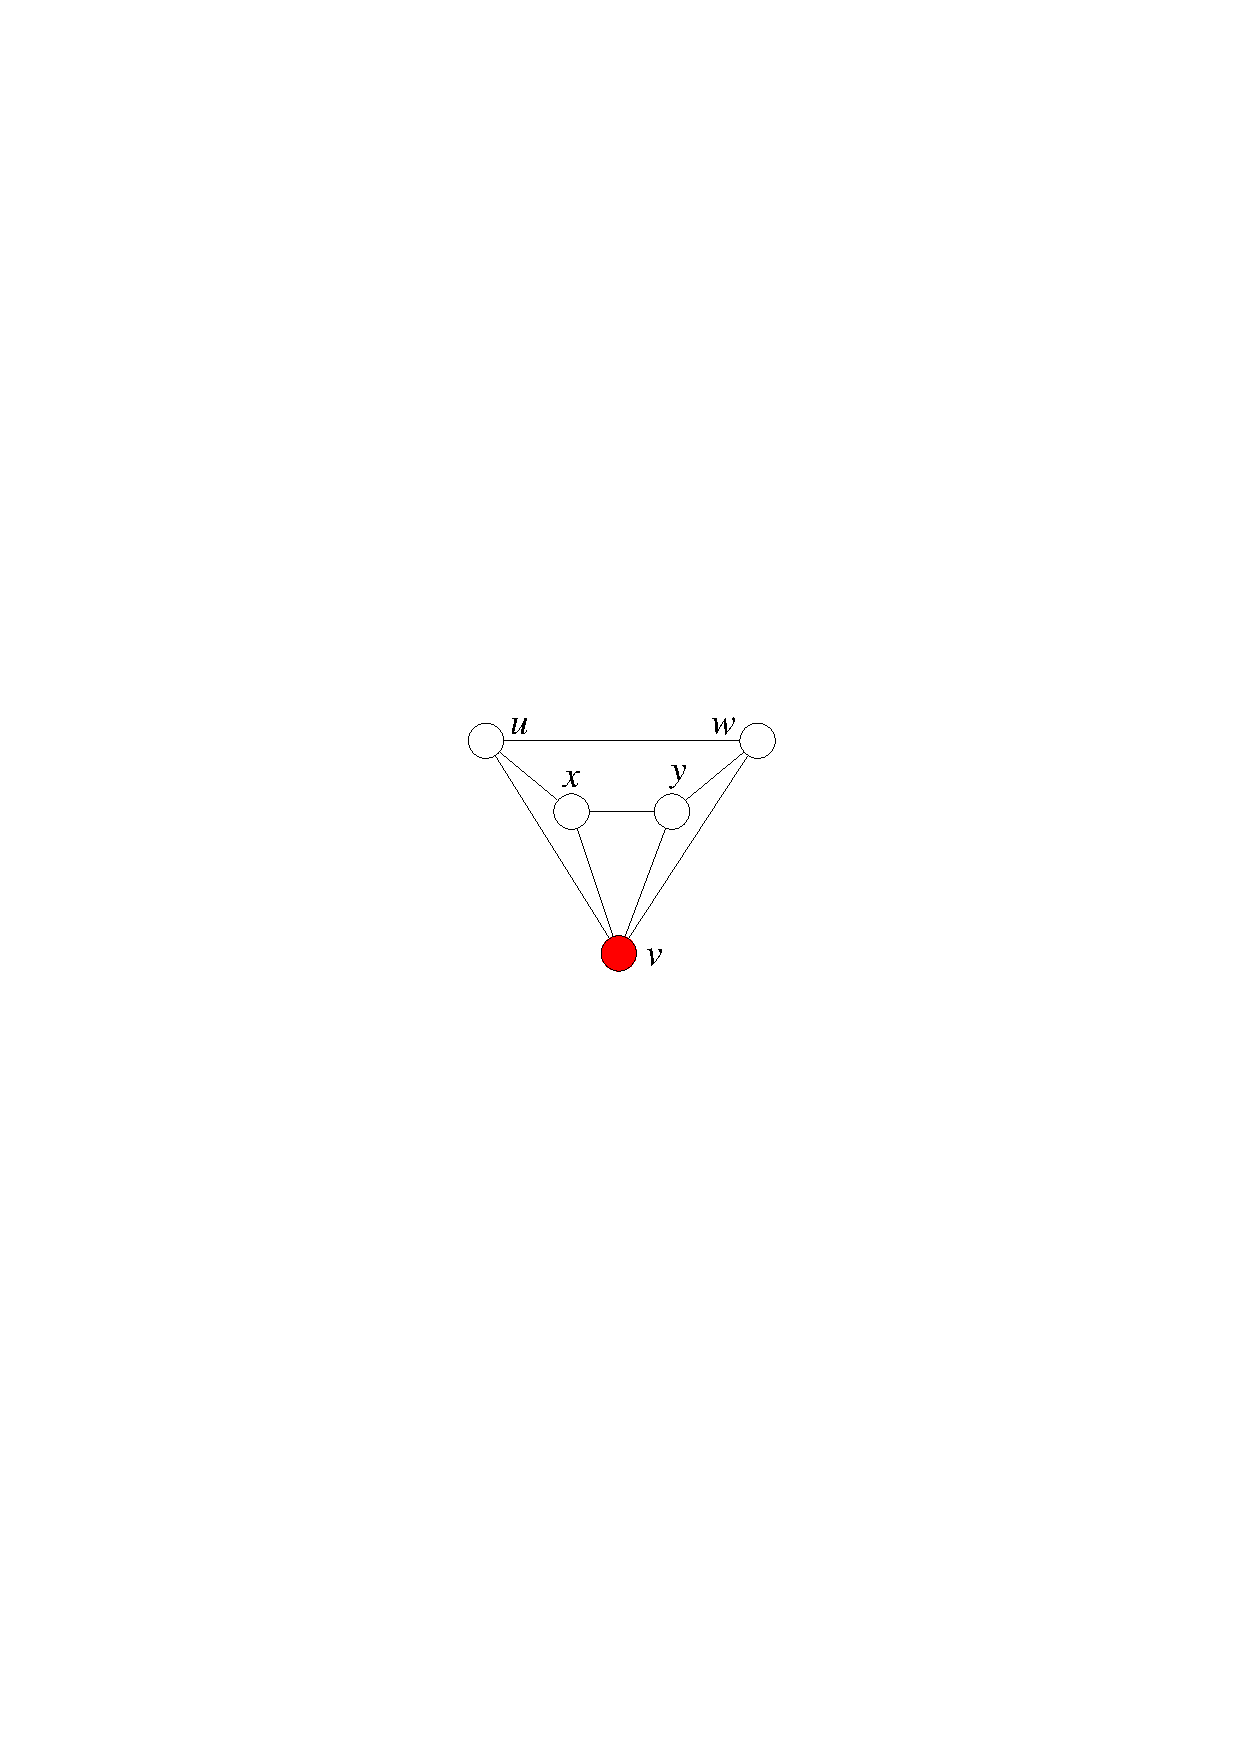
\includegraphics[width=.21\textwidth]{fig405-a}}
  \subfloat[结构II]{
    \label{fig:405b}
    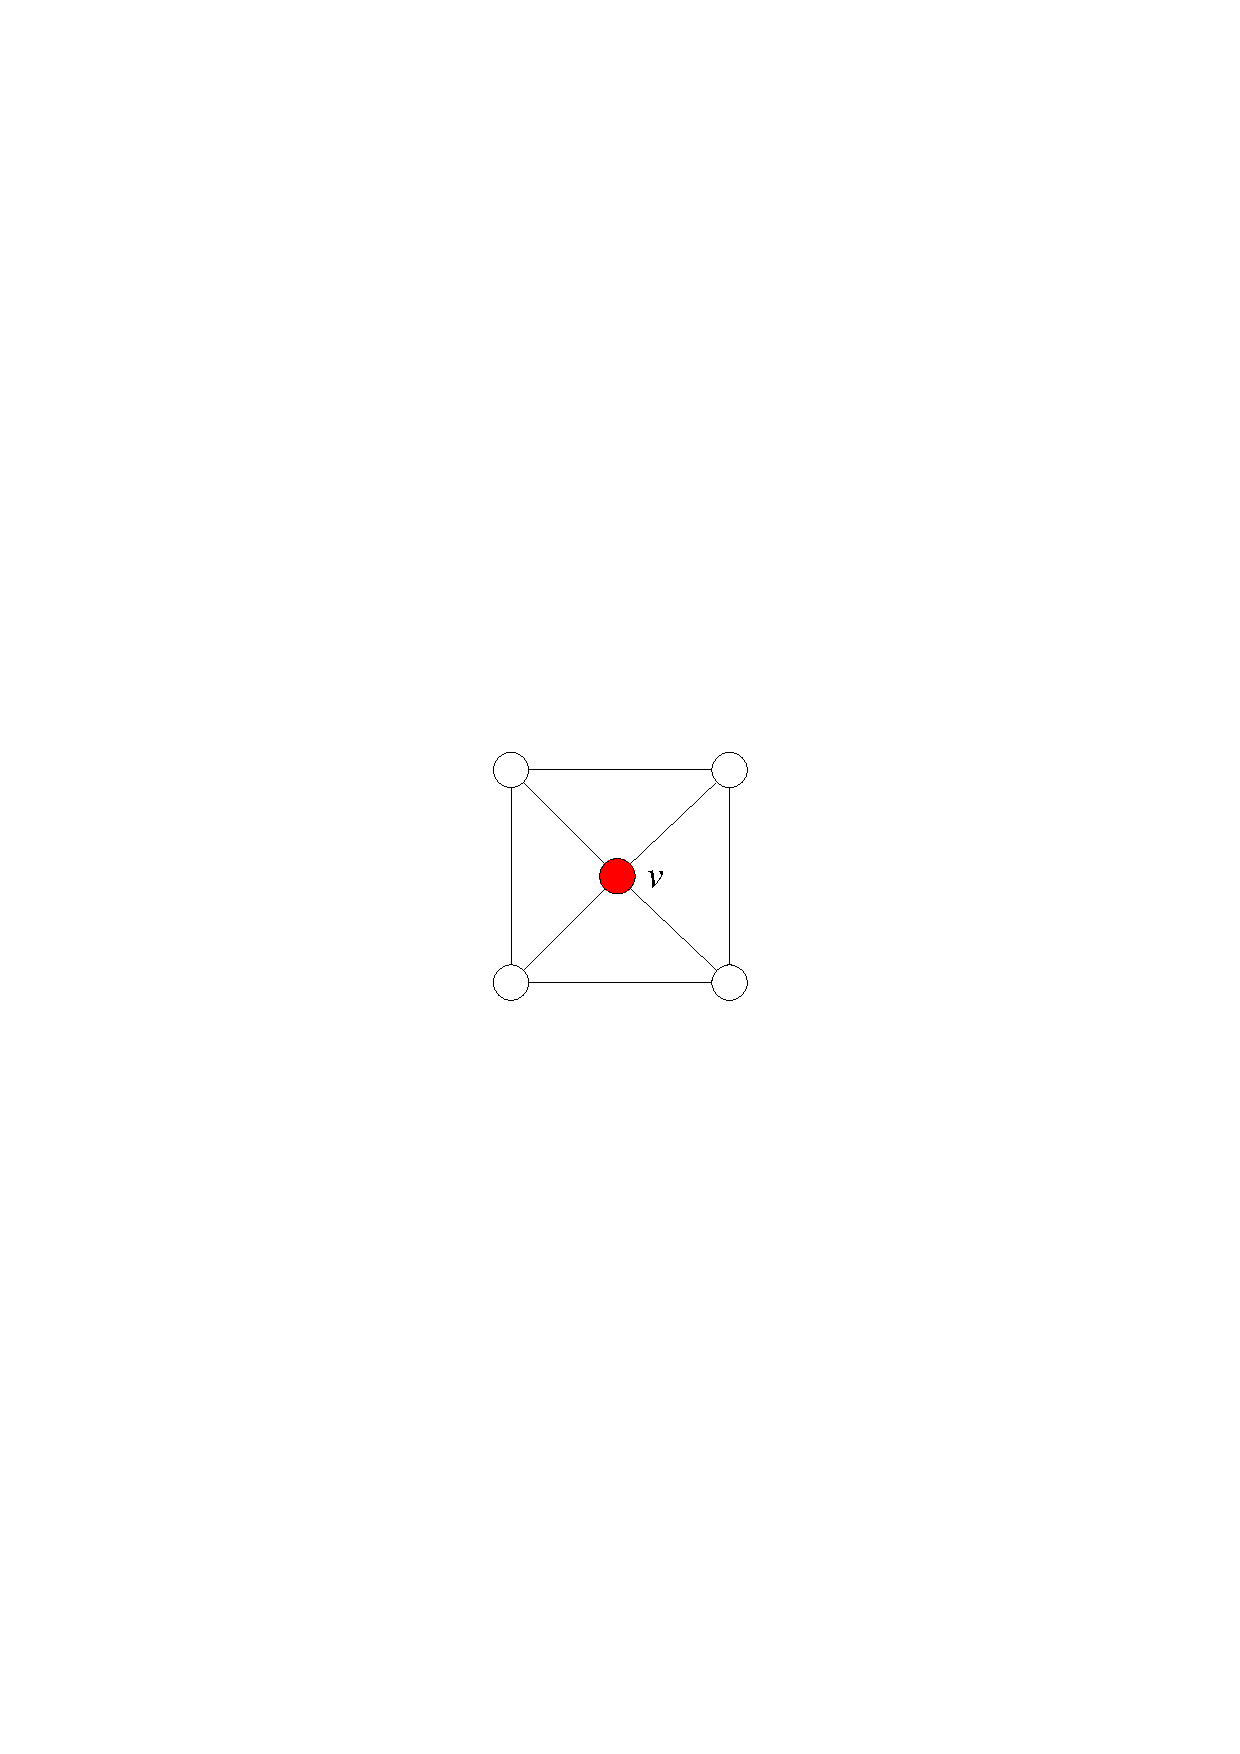
\includegraphics[width=.175\textwidth]{fig405-b}}
  \subfloat[结构I的实现]{
    \label{fig:405c}
    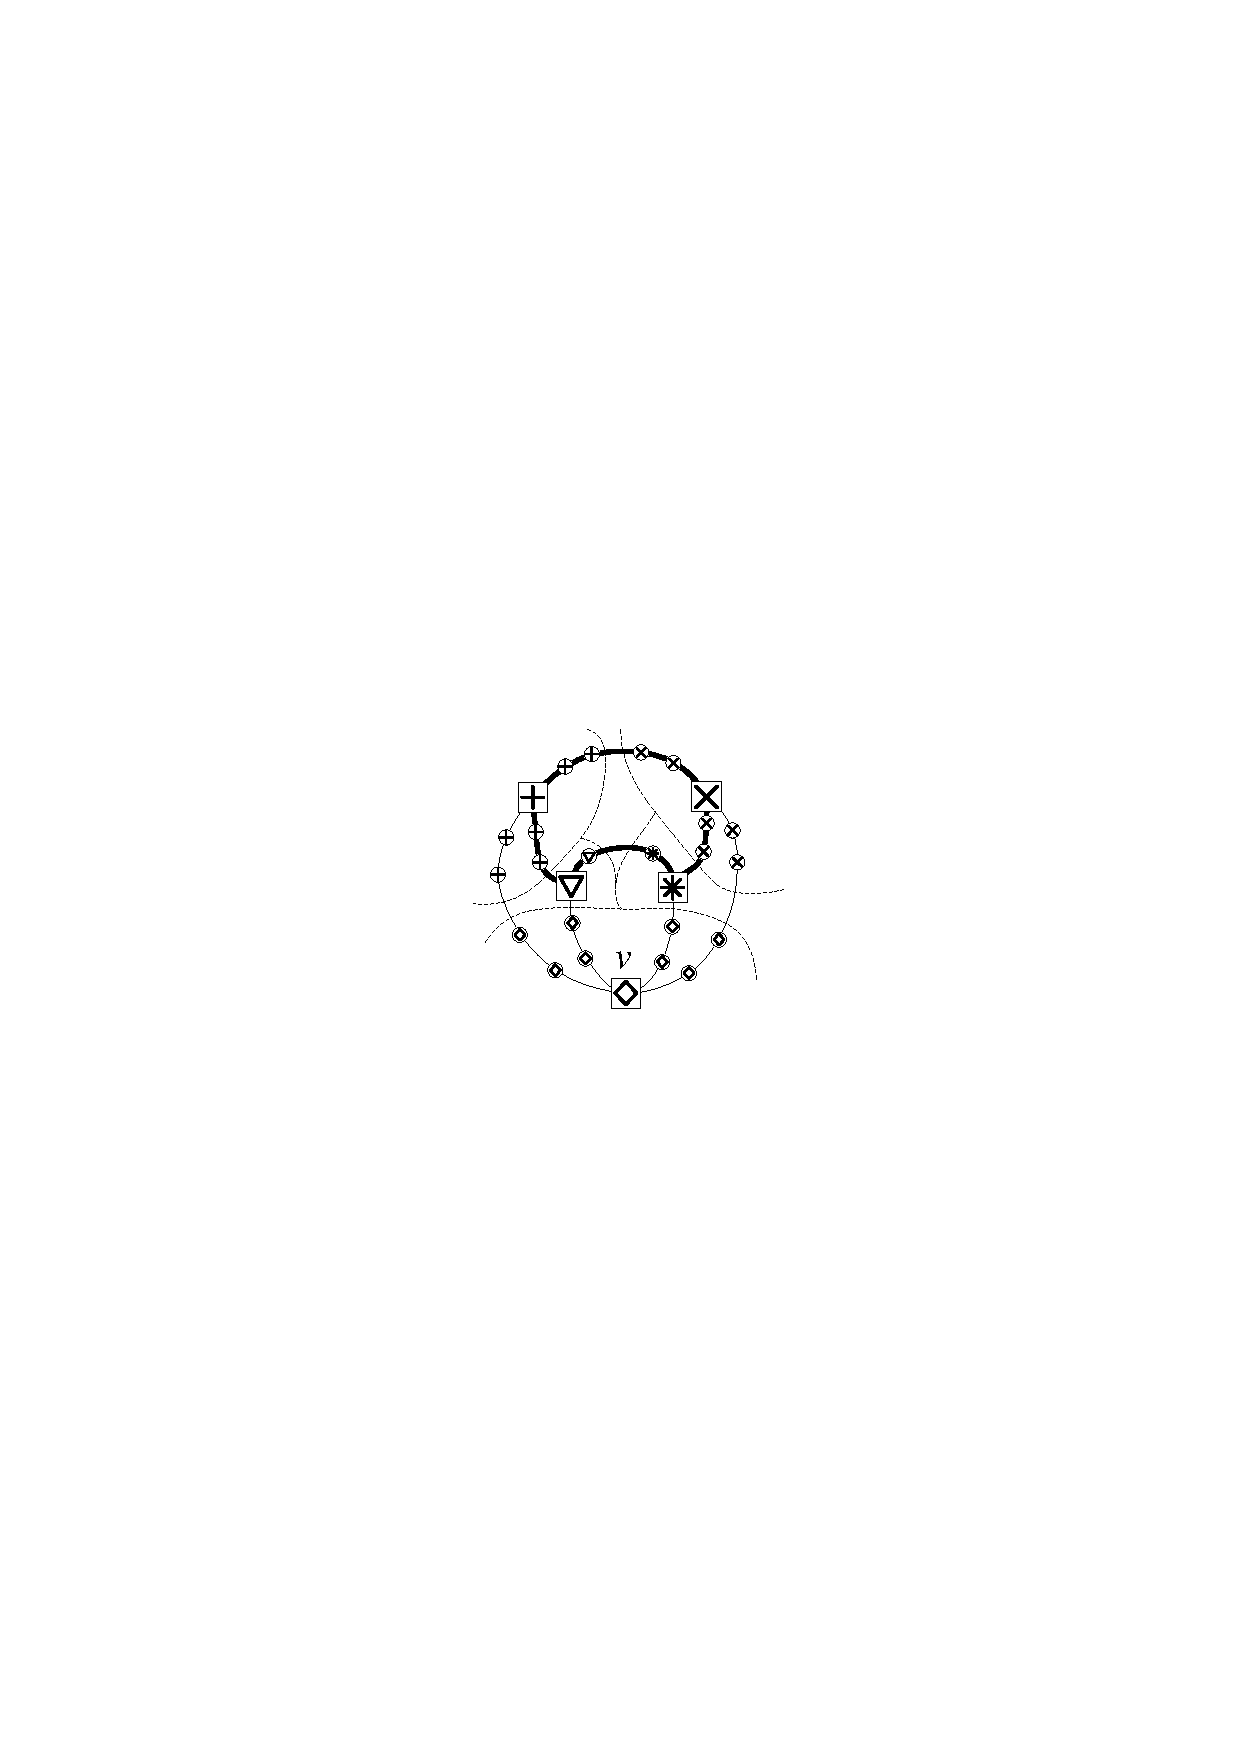
\includegraphics[width=.195\textwidth]{fig405-c}}
  \subfloat[对应的嵌入]{
    \label{fig:405d}
    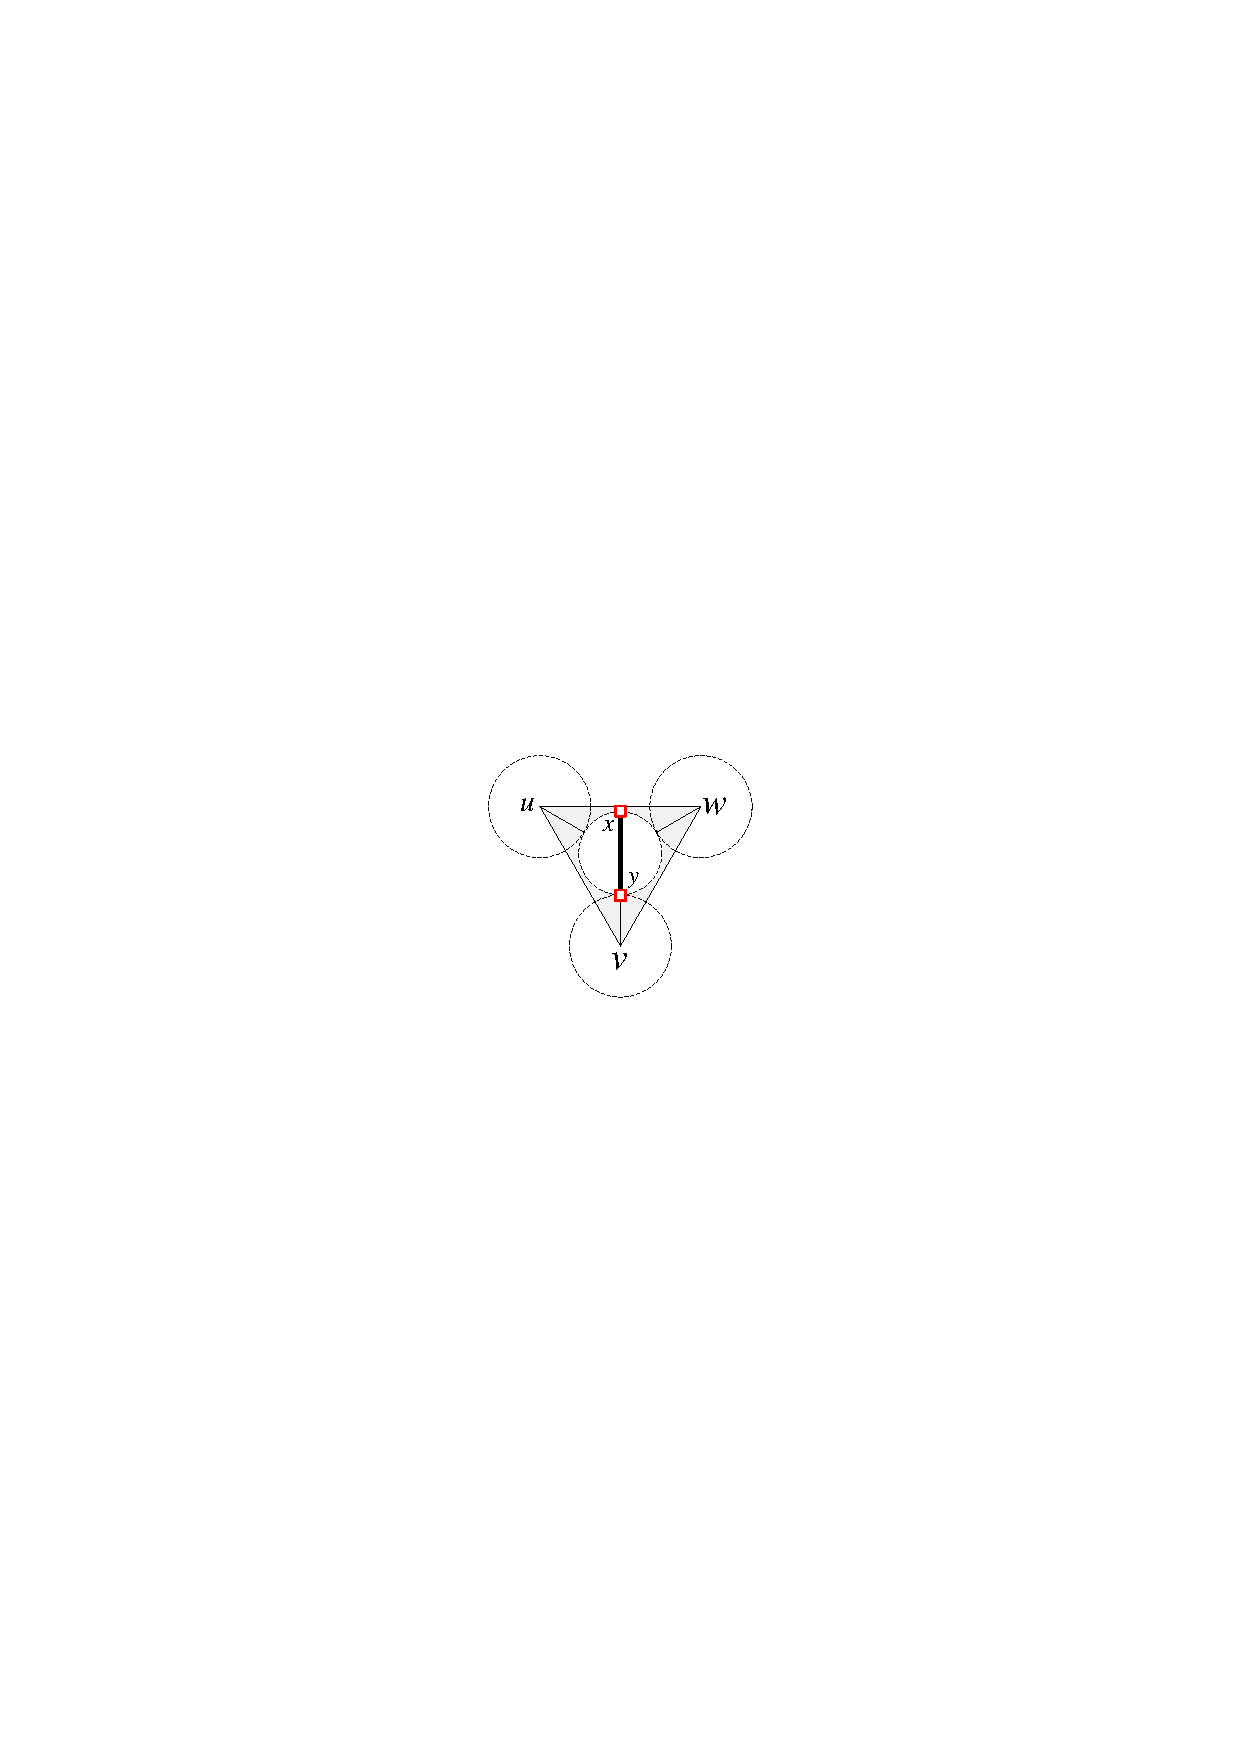
\includegraphics[width=.195\textwidth]{fig405-d}}
  \subfloat[结构III]{
    \label{fig:405e}
    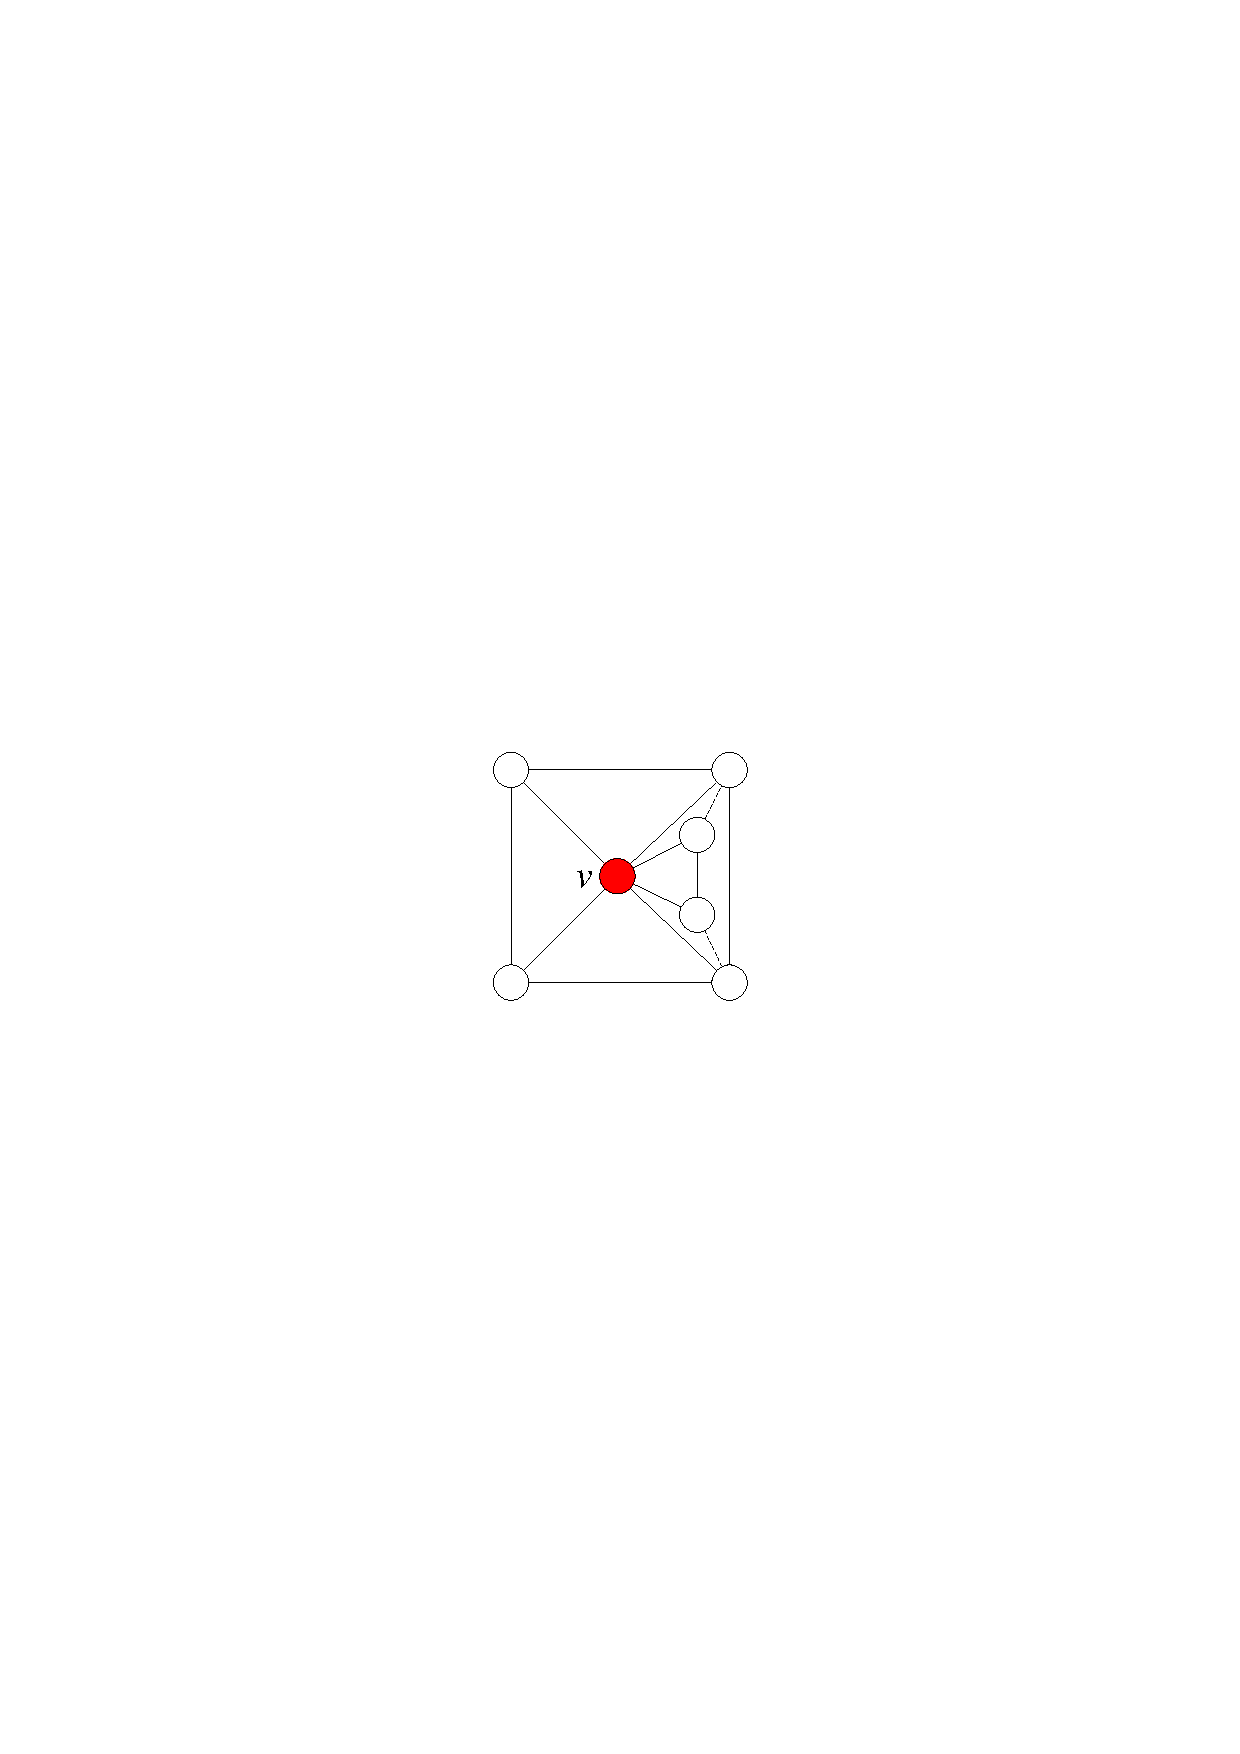
\includegraphics[width=.175\textwidth]{fig405-e}}
  \caption{RWG图中可能的结构}
  \label{fig:405}
\end{figure}

下面分析结构II的可实现性。因为$N_{\Gamma}^1(v)$中还包含两个不位于环$C$上、且直接相邻的顶点,为了实现顶点$v$、环$C$以及这两个额外顶点的平面化的嵌入,只有一种可能的情况,即图\ref{fig:405e}所示的结构III。显然,结构III中包含一个与结构I相同的子结构。前面已经证明了结构I的可实现性。因此,在UDG图模型和$\rho>5\sqrt{3}/18$的Q-UDG图模型下,结构II 也是不可能实现的。

综上所述,在UDG图模型和$\rho>5\sqrt{3}/18$的Q-UDG 图模型下,两个额外的相邻节点不可能在不破坏图的平面性的情况下嵌入到$N_{\Gamma}^1(v)$中一个长度为4 的环中。当环的长度增加时,这一结论始终成立。其证明过程类似,这里不再赘述。
\end{proof}
\subsection{修正过程}
在局部可平面性检验组件中检测出所有的疑似虫洞节点后,WormPlanar执行修正过程,以移除可能存在的误报的情况。在深入分析虫洞链路对网络的连通性造成的本质影响的基础上,我们提出了判定虫洞链路的两条必要条件,分别如定理\ref{theorem404}和定理\ref{theorem405}所述。假设点集$X$和$Y$分别表示位于两端的虫洞节点集合,边集$X\times{Y}$表示分别位于两端的的虫洞节点之间的虫洞链路集合。给定初始的网络连通图$G$,图$G^{'}$表示由点集$X\cup{Y}$和边集
$X\times{Y}$形成的$G$的子图,图$G^{''}$表示从$G$ 中删除$X\times{Y}$中所有边得到的子图。$\delta$表示所要检测的虫洞长度的下限。

\begin{theorem}
  \label{theorem404}
图$G^{'}$是图$G$中的一个极大完全二部子图。
\end{theorem}
\begin{proof}
因为点集$X$和$Y$分别包含虫洞两端的虫洞节点,在任意的节点$x\in{X}$看来,自己能够与虫洞另一端的所有虫洞节点直接通讯。因此,$x$与任意的节点$y\in{Y}$ 之间存在一条边,反之亦然。图\ref{fig:401b} 给出了虫洞节点构成的拓扑结构的一个实例。显然,$G^{'}(X\cup{Y},X\times{Y})$将构成一个完全二部图。向$X$或$Y$中加入任意一个正常节点,将无法与另一端的所有虫洞节点之间建立直接的链路。因此,图$G^{'}$是图$G$中的一个极大完全二部子图。
\end{proof}

\begin{theorem}
  \label{theorem405}
设$\theta$为一个正整数,且满足$\theta=\lfloor\delta/2\rfloor$。在满足虫洞长度下限的情况下,任意的两个节点$x\in{X},y\in{Y}$各自的$\theta$跳邻居集合不包含相同的元素,即$N_{G^{''}}^{\theta}(x)\cap{N_{G^{''}}^{\theta}(y)}=\emptyset$。
\end{theorem}
\begin{proof}
假设存在节点对$x\in{X},y\in{Y}$,满足$N_{G^{''}}^{\theta}(x)\cap{N_{G^{''}}^{\theta}(y)}\not=\emptyset$。 那么,节点$x$和$y$之间的最短距离一定不大于$2\theta$,即$d(x,y)\le{2\theta}$。那么,点集$X$ 和$Y$之间的距离也一定不大于$2\theta$,即$d_{G^{''}}(X,Y)\le2\theta\le\delta$,这与所要检测的虫洞长度的下限相矛盾。因此得到$N_{G^{''}}^{\lambda}(x)\cap{N_{G^{''}}^{\lambda}(y)}=\emptyset$。
\end{proof}

定理\ref{theorem404}和定理\ref{theorem405}被利用来过滤疑似虫洞节点。首先,从图$G$中找出所有的由疑似虫洞节点组成的连通组件,孤立的疑似虫洞节点将被排除。假设$\mathcal{S}$表示所有连通组件构成的集合。然后,从这些连通组件中找出所有的极大完全二部子图。为了提高检测率,我们将每个连通组件扩展至它们的1跳邻居,即将连通组件中的节点的1跳邻居节点加入该连通组件。这样,一旦该组件包含了位于虫洞两端的各一个节点,所有的虫洞节点都将被包含至该组件中。文献\upcite{bipartite}中查找所有极大完全二部子图(MCBS)的算法被应用于每个连通组件$S\in{\mathcal{S}}$。假设$\mathcal{B}$表示查找出的所有的极大完全二部子图的集合,$B=(W_0,W_1)$表示$\mathcal{B}$中的一个元素,其中$W_0$和$W_1$分别表示二部图$\mathcal{B}$两侧的顶点集合。至此,根据定理\ref{theorem404},所有不属于$\mathcal{B}$中的疑似虫洞节点将被排除。接下来,利用定理\ref{theorem405}对剩下的疑似虫洞节点进行进一步的过滤。为了排除多虫洞情况的干扰,我们仅将非疑似虫洞节点作为有效的邻居。对于每一个$B\in{\mathcal{B}}$,如果$N_{G^{''}}^{\lambda}(W_0)\cap{N_{G^{''}}^{\lambda}(W_1)}=\emptyset$,则$B$中的节点被确认为虫洞节点。否则,将$B$从$\mathcal{B}$中移除,并排除$B$中所有的疑似虫洞节点。至此,我们得到了最终的虫洞节点的检测结果。

另外,WormPlanar方法的最终目标是在不影响正常的网络功能的情况下消除虫洞效应,即在保持节点正常功能的基础上隔离虫洞链路。由于所有的虫洞节点都被准确地定位,我们可以简单地通过隔离两端的虫洞节点之间的虫洞链路来实现这一目标。
\begin{algorithm}[t]
\caption{WormPlanar算法}
\label{alg:401}
\begin{algorithmic}[1]
\REQUIRE ~~\
网络连通图$G(V,E)$
\ENSURE ~~\
检测出的虫洞节点集合$D$
\STATE 初始化虫洞集合为空集$D=\emptyset $;
\FOR {任意一个节点$v\in{V}$}
    \STATE 获得$v$的$k$跳邻居子图$G_k(v)$;
    \STATE 对$G_k(v)$应用平面化算法TPS,得到$\Gamma(v)$;
    \STATE 验证$\Gamma(v)$的平面性;
    \IF {$\Gamma(v)$是非平面图}
        \STATE 将$v$加入疑似虫洞节点集合$P$;
    \ENDIF
\ENDFOR
\STATE 从$G$中找出$P$中节点构成的连通组件集合$\mathcal{S}$;
\FOR {任意一个$C\in{\mathcal{C}}$}
    \STATE 从$C$中找出所有的极大完全二部子图$B$;
    \STATE 将$B$加入极大完全二部子图集合$\mathcal{B}$;
\ENDFOR
\FOR {$\mathcal{B}$中的任意一个$B=(X,Y)$}
    \IF {$N_{G^{''}}^k(X)\cap{N_{G^{''}}^k(Y)}\not=\emptyset$}
        \STATE 将$B$从$\mathcal{B}$中移除;
    \ENDIF
\ENDFOR
\STATE 将$\mathcal{B}$中所有的节点加入集合$D$,输出$D$;
\end{algorithmic}
\end{algorithm}
\subsection{算法与讨论}
完整的WormPlanar虫洞检测算法如算法\ref{alg:401}所述。下面分析算法中几个关键的参数以及它们对算法性能的影响,并讨论算法的复杂度。
\subsubsection{算法参数分析}
首先分析参数$k$的影响,即每个节点收集的局部邻居子图的范围。如果$k$取一个非常小的值(如$k$=3),虫洞节点的平面化处理结果中将可能无法形成环,导致其非平面性无法被检测到,从而影响算法的检测率。$k$取值较大时,又将导致算法的复杂度显著增加。一般情况下,$k$=5是一个比较合理的值。本章后面还将通过具体的仿真实验对这一问题进行验证。

另外一个影响WormPlanar性能的重要参数是节点分布特性,包括节点部署模型和节点密度。直观上,WormPlanar算法在均匀、稠密部署的网络中将提供更好的检测性能。因为在这种网络情况下,虫洞造成的非平面性特征将更明显,也更容易被检测出。具体来讲,在虫洞节点的平面化处理结果中将更容易形成环,这将提高WormPlanar算法检测的成功率。后面的实验部分也将对这一参数进行具体的验证。

最后讨论虫洞位置的影响。WormPlanar算法要求在虫洞节点的平面化结果中至少形成一个环结构。如果虫洞的两端都位于网络的边界,则无法满足该要求。因此,WormPlanar算法无法处理这种特殊情况。但是实际上,这种特例很少出现,且现有的大部分基于连通性信息的虫洞检测方法均无法处理这种特例。另外,当网络中存在多个具有任意相对位置的虫洞时,现有的其它基于连通性信息的检测方法均无法处理,而WromPlanar算法依然能够有效地处理。因为在这种情况下,网络的非平面化特征反而更明显,而不会影响WormPlanar算法的有效性。

\subsubsection{算法复杂度分析}
下面对WormPlanar算法的复杂度和可扩展性进行分析。

首先,在局部可平面性检验组件中,整体的开销主要包括两部分。第一部分是节点收集$k$跳邻居子图带来的开销。这部分功能可以通过所有节点发送一个局部的洪泛消息来实现,该过程中消息复杂度的上限为$\mathcal{O}(\Delta^{k+2})$,其中$\Delta$表示网络中节点度的最大值。第二部分的开销来自于每个节点对邻居子图应用平面化算法。按照文献\upcite{planar_infocom11}给出的结果,平面化算法的时间复杂度为$\mathcal{O}(\max\{\log\Delta\log^*n^{'},\Delta^{\tau+2}\})$,其中$n^{'}$表示邻居子图中节点的数量,$\tau$表示在构建RWG图时生成的$\tau$跳极大独立集。本章中始终取$\tau$=2。因此,当网络的最大节点度$\Delta$存在常数上限时,对于固定的$k$值,局部可平面性检验组件总的时间复杂度降低为$\mathcal{O}(\log^*n^{'})$。

其次,修正过程的开销主要来自于极大完全二部子图的查找算法。这一部分功能可以通过将疑似虫洞节点的连通性信息聚合至某一节点,并由该节点独立地完成计算。按照文献\upcite{bipartite}中的讨论,这一算法的复杂度的上限为$\mathcal{O}(a^32^{2a}n_s)$,其中$n_s$表示疑似虫洞节点的数量,$a$表示所有疑似虫洞节点组成的子图的荫度(arboricity)。$n_s$的值由实际的虫洞节点的数量决定。实际的虫洞节点越多,由于靠近虫洞节点而被误判为疑似虫洞节点的正常节点越多。而$n_s$的上限值为$n_w(d^{k+1}-1)/(d-1)$,其中$d$表示子图$G_s$的平均节点度。图的荫度表示图中所有的边可以被划分成的森林的最小数量,而荫度值的上限为$1+\lceil\Delta/2\rceil$\upcite{arboricity}。 因此,当最大节点度$\Delta$ 和实际的虫洞节点数量都存在常数上限时,修正过程的总的算法复杂度降低为$\mathcal{O}(d^{k+1})$。

综上所述,WormPlanar算法的总体复杂度主要由局部邻居子图的范围和实际的虫洞节点的数量决定,而与全局网络的规模无关。因此,WormPlanar算法具有良好的可扩展性,可以有效地应用于任意规模的网络。
\section{实验评估}
本节通过大量的仿真实验来评估WormPlanar算法在不同网络条件下的有效性和性能,并与目前已有的其它主要方法进行对比和分析。实验主要对三个性能指标进行评估,分别是检测率、误报率,以及多虫洞情况的检测,并对几个主要的参数及其对算法性能的影响进行分析。
\subsection{实验设置}
在仿真实验中,我们将验证WormPlanar算法在多种不同网络设置下的有效性和性能,如节点部署模型和节点密度、通讯图模型,以及虫洞位置。节点部署模型采用扰动网格模型和随机部署两种方式。节点的平均密度通过调整通讯半径来调节,平均节点度的变化范围在5至20之间。虽然理论分析显示WormPlanar算法对通讯模型没有特别的要求,但为了验证这一结论,我们仍对算法在不同的通讯图模型下的性能进行了测试。另外,虫洞的位置是影响算法检测性能的一个重要因素,特别是当网络中存在多个虫洞时,它们之间的相对位置往往对检测算法的有效性产生决定性的影响。本节将对不同位置下的虫洞的检测,以及具有任意相对位置的多虫洞的情况进行评估。在整个仿真实验中,每一项测试都对100个独立、随机生成的网络进行测试并给出平均值。
\subsection{检测率}
首先对WormPlanar算法在不同网络设置下的检测率进行评测。检测率定义为成功检测出的虫洞节点的数量与实际的虫洞节点数量的比值。在仿真网络中,900个节点部署在正方形区域,一个长度大于8的虫洞被随机地部署在网络中。实际的虫洞节点数量的平均值大约等于20。图\ref{fig:406}给出了WormPlanar算法在不同的网络设置下的检测率的评测结果,其中$x$轴表示平均节点度的值,$y$轴表示检测率的平均值。对评测结果中不同参数的影响进行分析,可以得到如下几个重要的结论。
\begin{figure}[t]
  \centering
  \subfloat[扰动网格,UDG]{
    \label{fig:406a}
    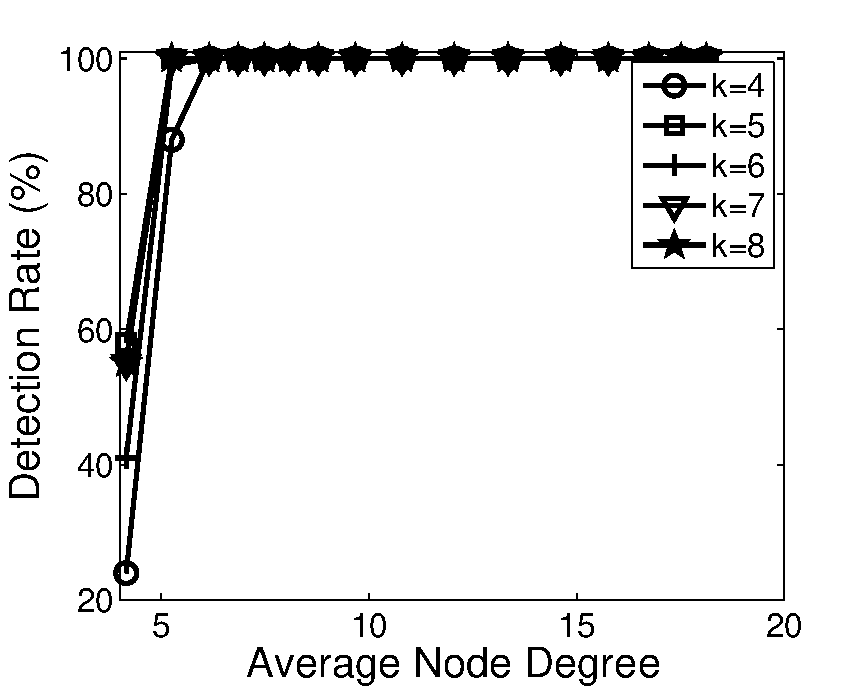
\includegraphics[width=.45\textwidth]{fig406-a}}\hspace{0.5em}%
  \subfloat[扰动网格,Q-UDG]{
    \label{fig:406b}
    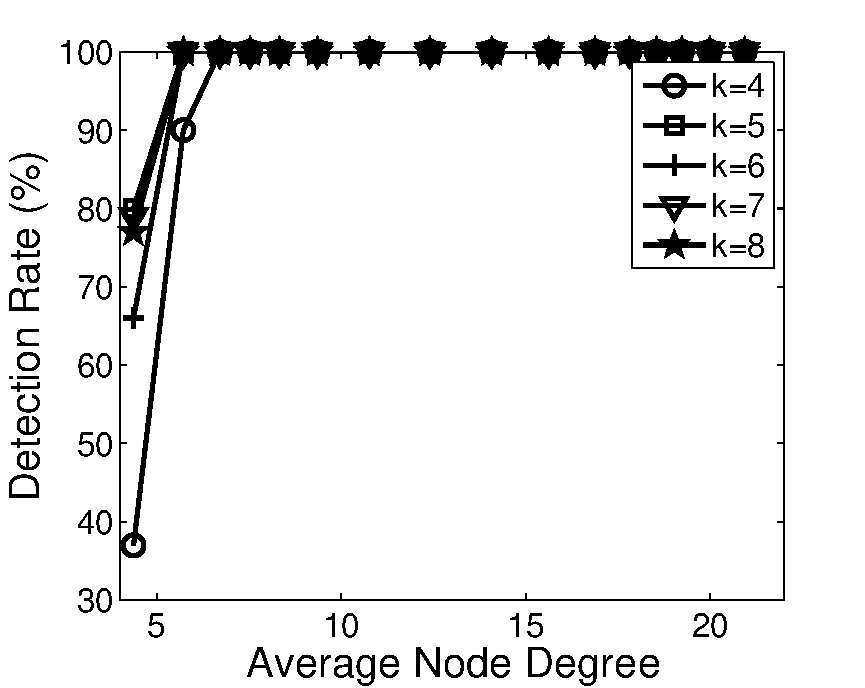
\includegraphics[width=.45\textwidth]{fig406-b}}\hspace{0.5em}%
  \subfloat[随机部署,UDG]{
    \label{fig:406c}
    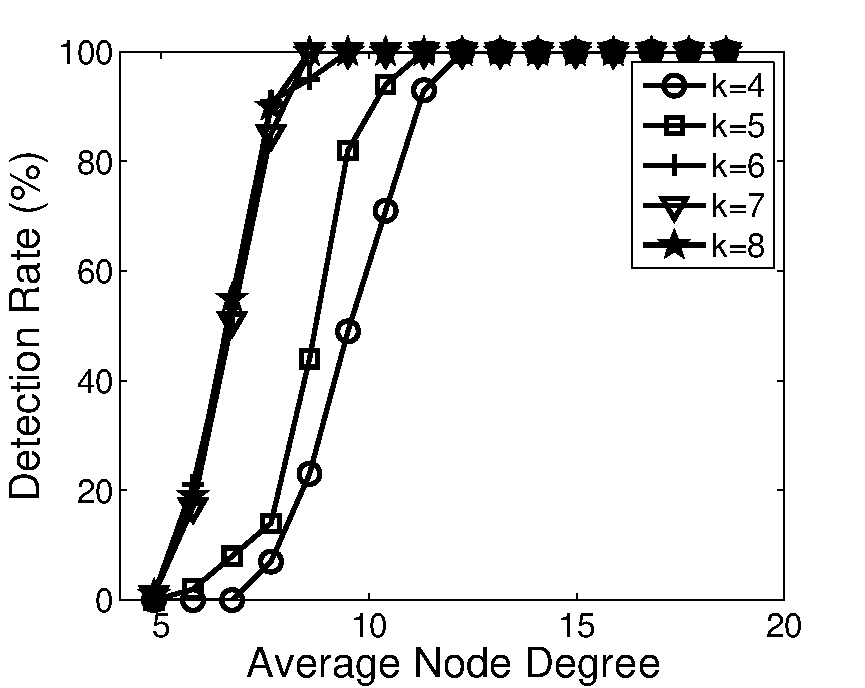
\includegraphics[width=.45\textwidth]{fig406-c}}\hspace{0.5em}%
  \subfloat[随机部署,Q-UDG]{
    \label{fig:406d}
    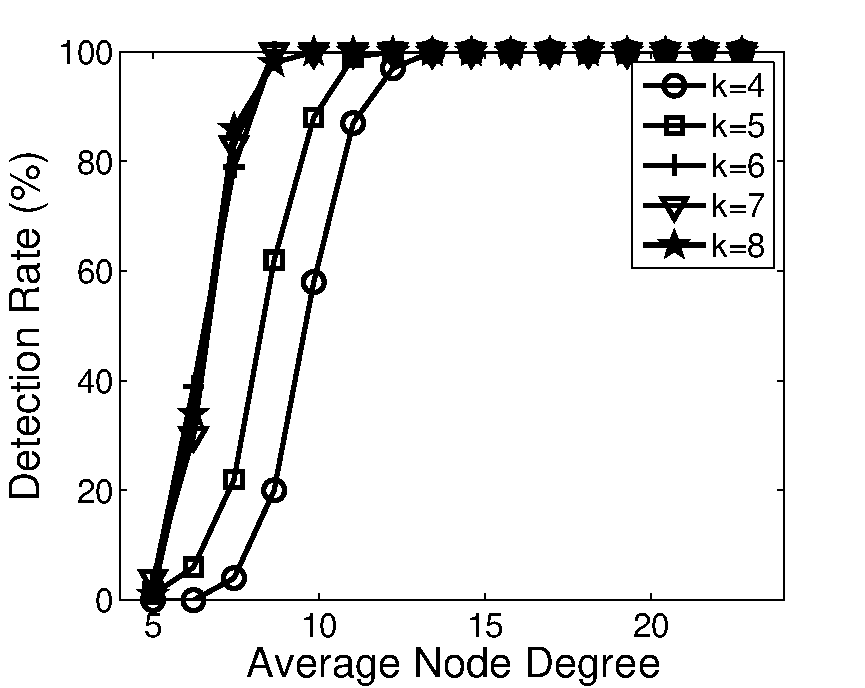
\includegraphics[width=.45\textwidth]{fig406-d}}
  \caption{WormPlanar算法在不同网络设置下的检测率}
  \label{fig:406}
\end{figure}
\subsubsection{节点密度的影响}
首先分析节点密度对WormPlanar算法检测率的影响。

实验结果显示节点密度对WormPlanar算法的检测率具有显著的影响。当平均节点度较低时,算法的检测率较低;当平均节点度增加时,算法的检测率也快速地提高。具体来讲,在扰动网格部署模型下,当平均节点度的值增加至大约6时,算法就能够成功地检测出所有的虫洞节点,即检测率达到100\%,如图\ref{fig:406a}-\ref{fig:406b}所示。在随机部署模型下,算法对节点度的要求稍高一些,当平均节点度的值增加至大约10 时检测率达到100\%,如图\ref{fig:406c}-\ref{fig:406d}所示。下面对出现这一结果的原因进行分析。

当节点度较低时,网络通讯图较稀疏。对于虫洞节点$v$,其局部邻居子图的平面化处理结果也比较稀疏,$v$的邻居地标节点将有可能无法形成环结构,从而导致算法无法识别出其非平面性特征,也就无法检测出该虫洞节点。而随着节点度的增加,这一现象将很快得到改善。节点度增加至一定的值后,所有的虫洞节点都能够被成功地检测出。
\subsubsection{节点部署模型和通讯图模型的影响}
下面分析节点部署模型和通讯图模型对WormPlanar算法的检测率的影响。

在节点部署模型方面,算法在扰动网格模型下的检测率(如图\ref{fig:406a}-\ref{fig:406b}所示)优于随机部署模型(如图\ref{fig:406c}-\ref{fig:406d}所示)。具体来讲,当平均节点度的值小于10时,算法在扰动网格模型下的检测率始终高于随机部署模型;平均节点度的值大于10时,算法在两种模型下的检测率都达到了100\%。出现这种结果的原因在于:在随机部署模型下,网络的不规则性较强,从而有可能导致虫洞节点的平面化处理结果中更难形成有效的环结构,因此算法检测的成功率低于扰动网格模型。但是这种影响仅限于网络密度较低的情况,当节点度增加至一定的值后,算法在两种模型下的检测率均达到了100\%。

在通讯图模型方面,实验结果显示算法在UDG模型(如图\ref{fig:406a}和\ref{fig:406c}所示)和Q-UDG模型(如图\ref{fig:406b}和\ref{fig:406d})下均获得良好的检测率性能。具体来讲,算法在UDG模型下的检测率略高于Q-UDG模型。这一微弱的差别可能源于UDG模型比Q-UDG模型产生的网络的均匀性稍好。
\subsubsection{邻居子图的范围的影响}
最后分析每个节点收集的邻居子图的范围(即算法中的参数$k$)对算法的检测率的影响。

实验结果显示,当$k$的取值较小时,检测率随着$k$值的增加而增加;当$k$的取值超过某个门限值后,检测率将不再受$k$值增加的影响。图\ref{fig:406a}-\ref{fig:406d}中所示的结果均符合这一规律。下面对产生这一结果的原因进行分析。当$k$的取值较小时(如$k$=3),虫洞节点的局部邻居子图的平面化处结果中难以形成有效的环结构,因此算法往往无法有效地检测出虫洞节点。当$k$的取值增加时,这一现象将很快得到改善。当$k$的取值超过某个门限值后,所有可能出现的环结构都已经形成,继续增加$k$的取值将不再对算法的检测率产生影响。相反,继续增加$k$的值将导致收集邻居子图带来的网络开销显著地增加。从实验结果来看,$k$=5是一个比较合适的取值,在大部分的网络实例中都能得到较好的结果。
\subsection{误报率}
下面对WormPlanar算法在不同网络设置下的误报率进行评测,并与LCT方法进行比较。误报率定义为被误判为虫洞节点的正常节点的数量与实际的虫洞节点数量的比值。我们仍采用与前面的检测率评测部分相同的网络设置,并统一要求两种算法均必须能够检测出长度大于8的虫洞。图\ref{fig:407}给出了WormPlanar算法及LCT算法在不同的网络设置下的误报率的评测结果,其中$x$轴表示平均节点度的值,$y$轴表示误报率的平均值。
\begin{figure}[t]
  \centering
  \subfloat[扰动网格,UDG]{
    \label{fig:407a}
    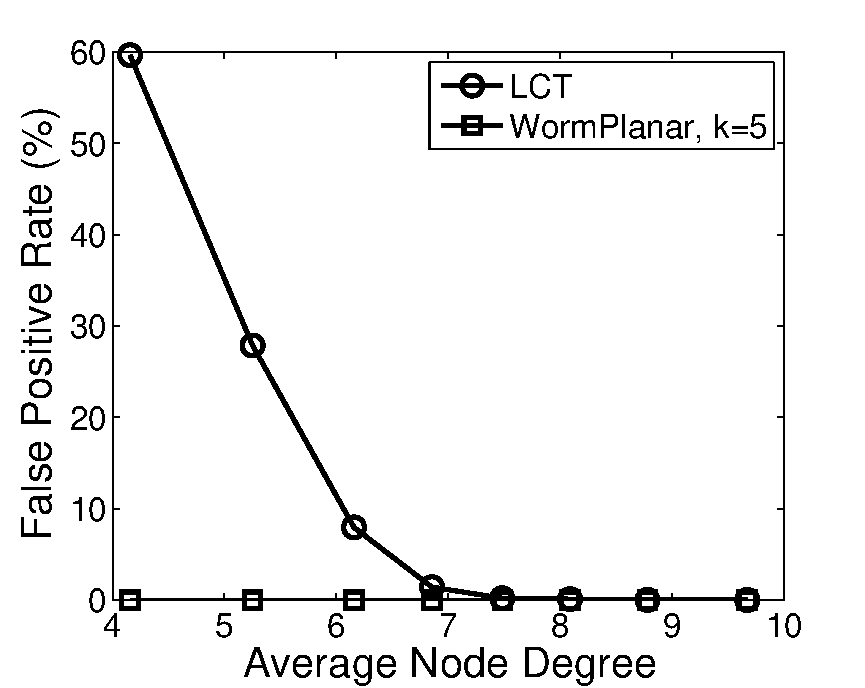
\includegraphics[width=.45\textwidth]{fig407-a}}\hspace{0.5em}%
  \subfloat[扰动网格,Q-UDG]{
    \label{fig:407b}
    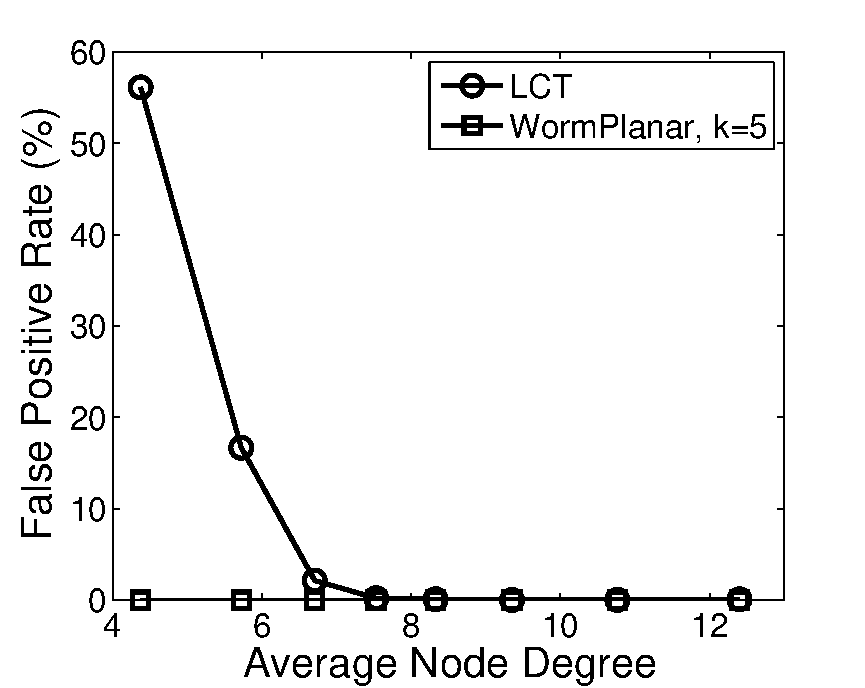
\includegraphics[width=.45\textwidth]{fig407-b}}\hspace{0.5em}%
  \subfloat[随机部署,UDG]{
    \label{fig:407c}
    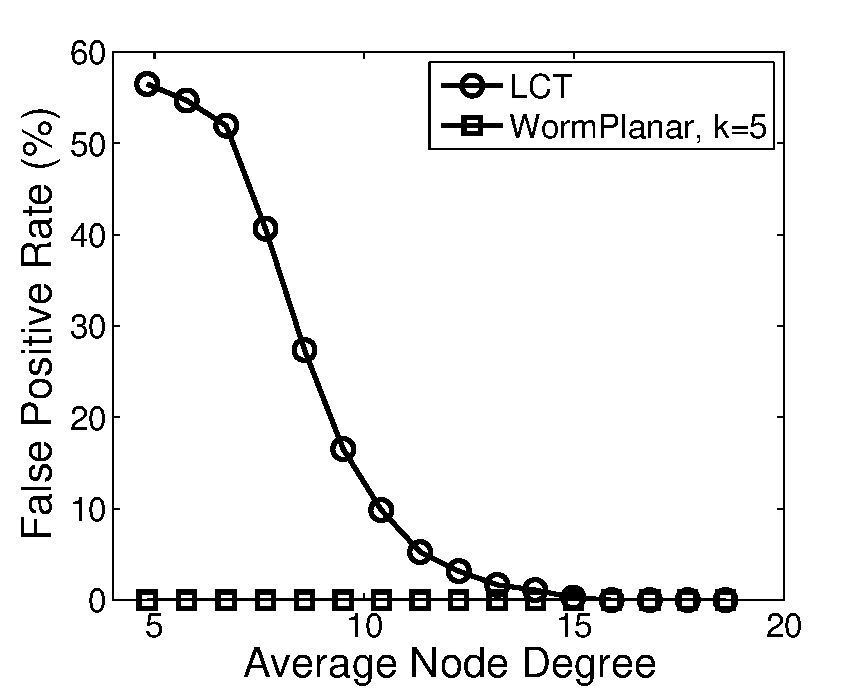
\includegraphics[width=.45\textwidth]{fig407-c}}\hspace{0.5em}%
  \subfloat[随机部署,Q-UDG]{
    \label{fig:407d}
    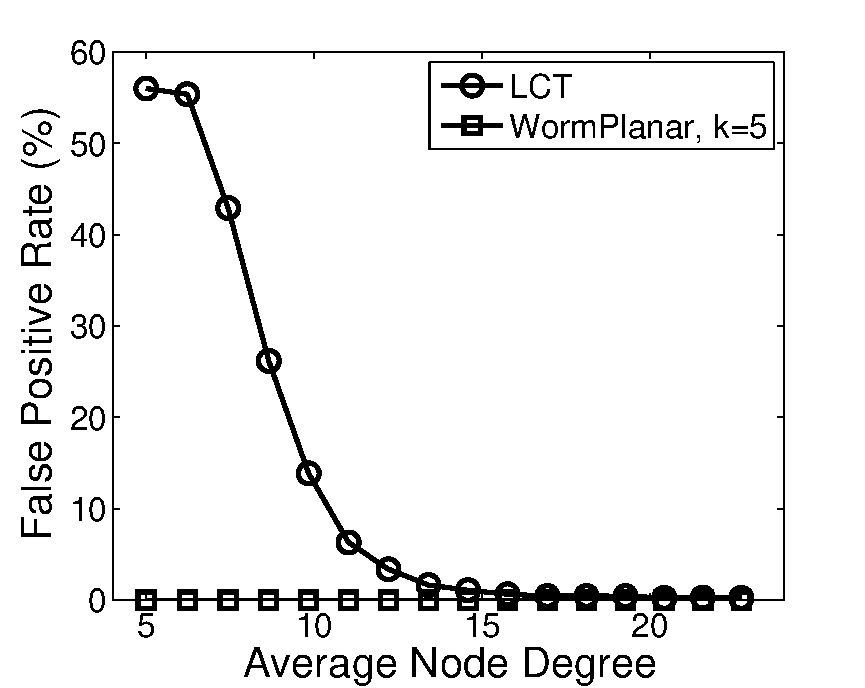
\includegraphics[width=.45\textwidth]{fig407-d}}
  \caption{WormPlanar及LCT算法在不同网络设置下的误报率}
  \label{fig:407}
\end{figure}

实验结果显示,WormPlanar算法在所有的网络设置下,均不存在误报的情况,而LCT算法则表现出较高的误报率,特别是在节点度较低或随机部署的网络中尤其明显。LCT算法虽然能够保证检测出所有的虫洞节点,但是同时产生的较多的误报将导致大量的正常链路被当作虫洞链路进行隔离,从而显著地影响网络整体的连通性和网络能力。虽然LCT算法可以通过增加局部连通性检验的范围来降低检测的误报率,但这将导致LCT算法能够检测出的虫洞长度的下限增加(即仅能检测到比较长的虫洞),从而显著地限制了算法的能力和适用范围。同时,增加局部连通性检验的范围也将使算法的通讯和计算开销显著增加。因此,WormPlanar算法和LCT 算法具有各自的优势和适用范围,但WormPlanar算法在不同的网络条件下表现出更好的鲁棒性。
\begin{figure}[t]
  \centering
  \subfloat[WormPlanar算法]{
    \label{fig:408a}
    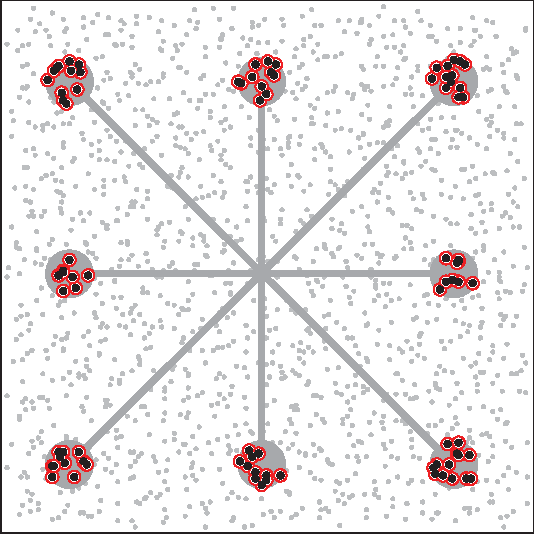
\includegraphics[width=.45\textwidth]{fig408-a}}\hspace{0.5em}%
  \subfloat[WormPlanar算法]{
    \label{fig:408b}
    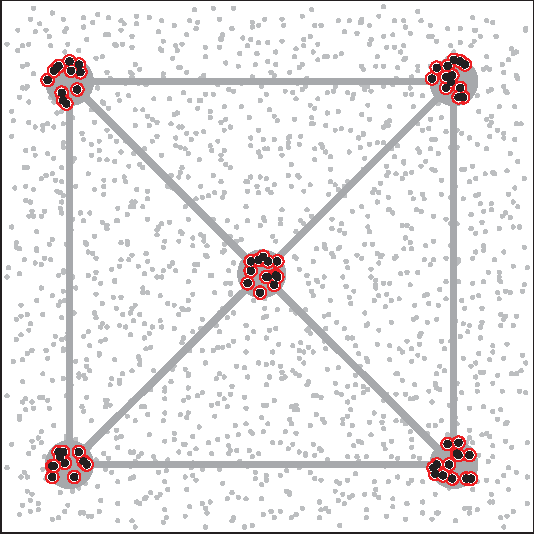
\includegraphics[width=.45\textwidth]{fig408-b}}\hspace{0.5em}%
  \subfloat[WormPlanar算法]{
    \label{fig:408c}
    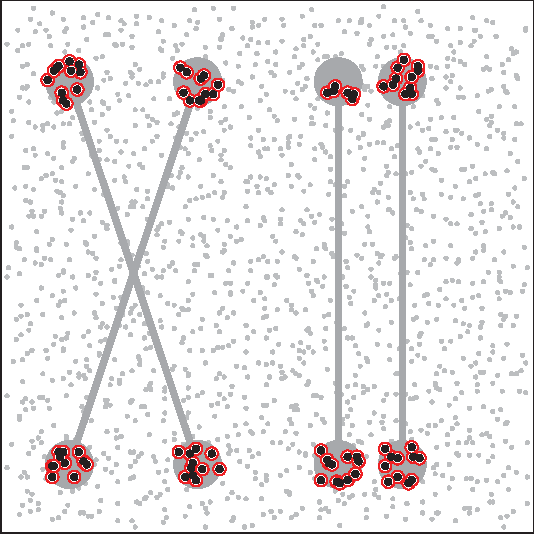
\includegraphics[width=.45\textwidth]{fig408-c}}\hspace{0.5em}%
  \subfloat[LCT算法]{
    \label{fig:408d}
    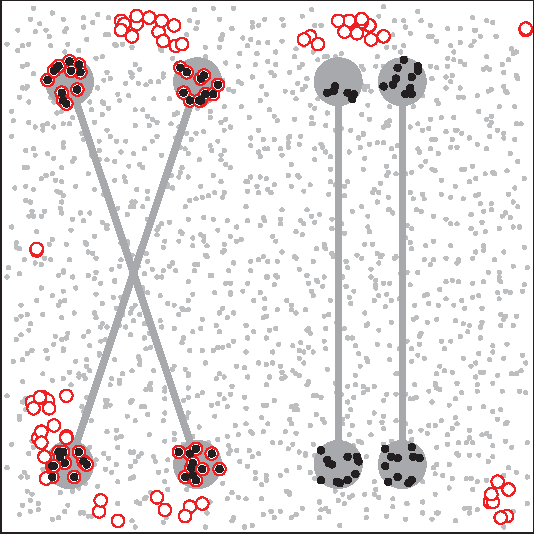
\includegraphics[width=.45\textwidth]{fig408-d}}
  \caption{WormPlanar及LCT算法对具有不同相对位置的多虫洞情况的检测}
  \label{fig:408}
\end{figure}

\subsection{多虫洞检测}
最后对WormPlanar算法在网络中存在多个虫洞的情况下的有效性进行评估,并与LCT方法进行比较,如图\ref{fig:408}所示。

当网络中存在多个虫洞时,虫洞之间将可能互相干扰,使得基于连通性信息的虫洞检测更加困难。特别是当它们处于某些特殊的相对位置时,可能导致检测算法完全失效。图\ref{fig:408a}-\ref{fig:408c}所示为WormPlanar算法对具有不同相对位置的多虫洞情况的检测结果,其中灰色区域表示虫洞天线的影响范围,黑点表示实际的虫洞节点,圆圈表示算法检测出的虫洞节点。可见WormPlanar算法可以准确地检测出图示网络中所有的虫洞节点。相对应地,图\ref{fig:408d}表示LCT 算法对图\ref{fig:408c}所示情况的检测结果。对于图中左侧的两个虫洞,LCT算法能够检测出所有的虫洞节点,但是同时也产生了很多的误报;而对于图中右侧的两个虫洞,LCT 算法则完全失效。下面出现这一结果的原因进行分析。对于图中右侧的两个虫洞,两端的虫洞节点之间的距离都比较近,因此同一个虫洞两端的节点将能够通过另一个虫洞内的虫洞链路建立连接,从而使得LCT算法中基于局部连通性的虫洞检测策略失效。WormPlanar算法之所以不受这种情况的影响,是因为算法将网络整体的非平面性特征作为检测虫洞的依据,而这一特征在网络中存在多个虫洞时并不会消失或减弱,甚至会更显著。同时,图\ref{fig:408}所示的实验结果也再次验证了WormPlanar算法在误报率方面的明显优势。
\section{本章小结}
虫洞攻击是无线自组织与传感器网中一种严重的攻击方式。虫洞攻击从根本上显著地改变了网络的拓扑结构,从而对很多基本的网络功能和协议造成严重的危害。现有的大部分虫洞检测方法依赖于特殊的硬件设备或理想的网络假设,从而限制了这些方法的可用性。而现有的基于网络连通性的检测方法都是基于利用离散域的局部的虫洞特征,或者连续域的全局的网络特征,而缺乏一种能够直接在离散域捕获虫洞造成的全局拓扑症状的检测手段。本文深入挖掘虫洞攻击对全局的拓扑结构造成的本质影响,发现了虫洞攻击对网络平面化造成的影响,并提出了一种仅利用局部连通性信息的虫洞检测方法,称为WormPlanar。WormPlanar首次实现了直接从离散域捕获虫洞造成的全局拓扑症状。本章从理论上充分地证明了WormPlanar方法的正确性,并通过大量的仿真实验对算法的性能进行验证,结果显示WormPlanr能够准确地检测和定位不同网络条件下的虫洞攻击,包括之前的基于连通性的检测方法均无法处理的多虫洞攻击。
